\documentclass[review]{elsarticle}

\usepackage{thumbpdf,lmodern}
\usepackage{amsmath}
\usepackage{color}
\usepackage{caption}
\usepackage{subcaption}
\usepackage{amssymb}
\usepackage{amsthm}
\usepackage{makecell}
\usepackage{verbatim}

\usepackage{lineno,hyperref}
\modulolinenumbers[5]

\journal{Fuzzy Sets and Systems}

%%%%%%%%%%%%%%%%%%%%%%%
%% Elsevier bibliography styles
%%%%%%%%%%%%%%%%%%%%%%%
%% To change the style, put a % in front of the second line of the current style and
%% remove the % from the second line of the style you would like to use.
%%%%%%%%%%%%%%%%%%%%%%%

% Numbered
% \bibliographystyle{model1-num-names}

%% Numbered without titles
% \bibliographystyle{model1a-num-names}

%% Harvard
% \bibliographystyle{model2-names}\biboptions{authoryear}

%% Vancouver numbered
% \usepackage{numcompress}\bibliographystyle{model3-num-names}

%% Vancouver name/year
% \usepackage{numcompress}\bibliographystyle{model4-names}\biboptions{authoryear}

%% APA style
% \bibliographystyle{model5-names}\biboptions{authoryear}

%% AMA style
% \usepackage{numcompress}\bibliographystyle{model6-num-names}

%% `Elsevier LaTeX' style, distributed in TeX Live 2019
\bibliographystyle{elsarticle-num}
% \usepackage{numcompress}\bibliographystyle{elsarticle-num-names}
% \bibliographystyle{elsarticle-harv}\biboptions{authoryear}
%%%%%%%%%%%%%%%%%%%%%%%

%\newenvironment{Schunk}{}{}
\newenvironment{Schunk}{\bgroup\linespread{1}}{\egroup}
\newenvironment{Sinput}{\endgraf\verbatim}{\endverbatim}
\newenvironment{Soutput}{\endgraf\verbatim}{\endverbatim}
\newcommand{\pkg}[1]{\textbf{#1}}
\newcommand{\proglang}[1]{#1}
\newcommand{\code}[1]{\texttt{#1}}

\newcommand{\lfl}{\pkg{lfl}}
\newcommand{\R}{\proglang{R}}
\newcommand{\todo}[1]{{\color{red} TODO: #1}}
\newcommand{\michal}[1]{{\color{green} MB: #1}}

\newcommand{\Martin}[1]{{\color{blue} Martin: #1}}

\newcommand{\tgodel}{{T}_{\textrm{M}}}
\newcommand{\tluk}{{T}_{\textrm{\L}}}
\newcommand{\tgoguen}{{T}_{\textrm{P}}}
\newcommand{\sgodel}{{C}_{\textrm{M}}}
\newcommand{\sgoguen}{{C}_{\textrm{P}}}
\newcommand{\sluk}{{C}_{\textrm{\L}}}
\newcommand{\rgodel}{{R}_{\textrm{M}}}
\newcommand{\rgoguen}{{R}_{\textrm{P}}}
\newcommand{\rluk}{{R}_{\textrm{\L}}}
\newcommand{\bgodel}{{B}_{\textrm{M}}}
\newcommand{\bgoguen}{{B}_{\textrm{P}}}
\newcommand{\bluk}{{B}_{\textrm{\L}}}
\newcommand{\ngodel}{{N}_{\textrm{M}}}
\newcommand{\ngoguen}{{N}_{\textrm{P}}}
\newcommand{\nluk}{{N}_{\textrm{\L}}}

\newcommand{\squ}{\mathop{\scriptstyle \square}\nolimits}
\newcommand{\dhd}{\mathop{\triangledown}\nolimits}

\newcommand{\RSE}{\mathop{(R\circ S^{\backprime}E)}\nolimits}

\def\lh{\mathop{\le_{\rm H} }\nolimits}

\newtheorem{rem}{Remark}

\newcommand{\T}{\text{\it T}}
\newcommand{\LD}{\text{\it LD}}
\newcommand{\Topic}{\text{\it Topic}}
\newcommand{\ExTop}{\text{\it ExTopic}}
\newcommand{\Focus}{\text{\it Focus}}
\newcommand{\LPerc}{\text{\it P}}
\newcommand{\lingterm}[1]{\text{\sf #1}}
\newcommand{\defeq}{\mathrel{:=}\,}
\newcommand{\LpredC}[2]{#1\text{ is }#2}
\newcommand{\Lpred}[2]{#2\ #1}
\newcommand{\IFRule}[4]{\lingterm{IF } \LpredC{#1}{#2}
\lingterm{ THEN } \LpredC{#3}{#4}}

\newcommand{\IFRuleMore}[6]{\lingterm{IF } \LpredC{#1}{#2} \lingterm{ AND
}\cdots \lingterm{ AND }\LpredC{#3}{#4} \lingterm{ THEN }
\LpredC{#5}{#6}}


\newcommand{\mlingterm}[1]{\langle\text{#1}\rangle}
\newcommand{\Core}{\mathop{\rm Core}\nolimits}
\newcommand{\Supp}{\mathop{\rm Supp}\nolimits}
\newcommand{\cov}{\mathop{\rm cov_{\LD}}\nolimits}
\newcommand{\covr}{\mathop{\rm cov_{\LD'}}\nolimits}
\newcommand{\red}{\mathop{\rm reduct_{\LD}^{\LD'}}\nolimits}

\def\Sm{\mathop{\rm Sm}\nolimits}
\def\Me{\mathop{\rm Me}\nolimits}
\def\Bi{\mathop{\rm Bi}\nolimits}
\def\lh{\mathop{\le_{\rm H} }\nolimits}
\def\llp{\mathop{\le_{x_0} }\nolimits}
%\def\llp{\mathop{\le_{(u_0,w)} }\nolimits}
\def\str {\mathop{<_{\rm LE} }\nolimits}
\def\lle{\mathop{\le_{\rm LE} }\nolimits}
\def\nlle{\mathop{\nleq_{\rm LE} }\nolimits}
\def\plle{\mathop{\parallel_{\rm LE} }\nolimits}
\def\lle{\mathop{\le_{\rm LE} }\nolimits}
\def\les{\mathop{<_{\rm LE} }\nolimits}



\begin{document}

\begin{frontmatter}

\title{lfl: Linguistic Fuzzy Logic in \R{} -- Part I}

%% Group authors per affiliation:
\author{Michal Burda\corref{corr}}\ead{Michal.Burda@osu.cz}
\author{Martin \v{S}t\v{e}pni\v{c}ka}\ead{Martin.Stepnicka@osu.cz}
\cortext[corr]{Corresponding author. Tel.: +420 59 709 1450; fax: +420 596 120 478.}
\address{Institute for Research and Applications of Fuzzy Modeling, University of Ostrava, CE~IT4Innovations, 30.~dubna 22, 701 03 Ostrava, Czech Republic}


\begin{abstract}
This paper presents an \R{} package that supports the use of fuzzy relational calculus and linguistic fuzzy logic in data processing applications. The \pkg{lfl} package enables computing compositions of fuzzy relations enhanced with distinct extensions, such as excluding features, unavoidable features, or generalized quantifiers. Furthermore, it provides tools for transformation of data into fuzzy sets representing linguistic expressions, mining of linguistic fuzzy association rules, and performing an inference on fuzzy rule bases using the Perception-based logical deduction (PbLD). The package also enables to use the Fuzzy rule-based ensemble, a tool for time series forecasting based on an ensemble of forecasts from several individual methods implemented in \R{}.
\end{abstract}

\begin{keyword}
fuzzy sets \sep fuzzy natural logic \sep linguistic fuzzy logic \sep association rules \sep compositions of fuzzy relations \sep\R{}
\end{keyword}

\end{frontmatter}

\linenumbers

\Martin{Utekly mi obrazky pod reference na konec clanku - nevim proc. \\ Premyslim nad tim delenim clanku na part I a Part II. Mozna pri zkraceni tech prikladu se to vejde do jednoho clanku. Porad totiz tapu, kde tu delici mezeru udelat a jak se v te druhe casti neopakovat. }

\section{Introduction} \label{sec:intro}


The aim of this paper is to present a new package for the \R{} statistical environment
\citep{R2020} that enables the use of the linguistic fuzzy logic in data processing
applications. The package provides implemented tools for using the results of original work of
\cite{Novak08, Novak:PbLD, DvoStep:PbLD2015, StepBurda:FRBE_FSS}, and others, and it provides
executable routines that are not freely available anywhere else.

Indeed, there already exist several packages for \R{} that are focused on vagueness and fuzziness. For
instance, the \pkg{sets}
package \citep{setsPkg} introduces many basic operations on fuzzy sets, the \pkg{FuzzyNumbers}
package \citep{FuzzyNumbersPkg} provides classes and methods to deal with fuzzy numbers,
the \pkg{SAFD} package \citep{safdPkg} contains tools for elementary statistics on fuzzy data, and
the \pkg{fclust} \citep{fclustPkg} brings the fuzzy K-Means clustering technique to the environment of
the \R{} system.

The \pkg{lfl} package described in this paper focuses on creation of systems based on fuzzy logic and their
usage in classification and prediction. A similar task is performed also by the \pkg{fugeR}
package \citep{fugeRPkg} that introduces an evolutionary algorithm for a construction of a fuzzy system from
a training data set, or by the \pkg{frbs} package \citep{frbsPkg} that provides many widely
accepted approaches for building the fuzzy systems, based on space partition, neural networks,
clustering, gradient descent, or genetic algorithms.

The algorithms provided by the \pkg{lfl} package are tightly connected with the notion of
the \emph{fuzzy natural logic} (FNL), formerly also called the \emph{linguistic fuzzy logic} (LFL),
that was initially developed by \cite{Novak08}. Moreover, it covers some other closely related areas, for example fuzzy relational calculus  (\cite{BandlerKohout78,Belohlavek_book2002,Behounek:Compositions})  that includes the latest generalizations (\cite{Cao2017, Cao2017b}), the algebraic structures for partial fuzzy logics (\cite{BehounekNovak:IEEE15, BehounekDankova:IPMU16}), and the connection of both topics (\cite{Step_etal_Dragon_IJAR2019}).

\emph{Evaluative linguistic expression} -- a central notion of the fuzzy natural logic -- is the expression of the form
%
$$\langle \textrm{linguistic hedge}\rangle \langle \textrm{atomic expression}\rangle$$
%
that vaguely evaluates a position on the real line, for example, \emph{``very small''}, \emph{``roughly medium''}, or \emph{``extremely big''}. The atomic expression takes values usually from the triplet 
\emph{``small''}, \emph{``medium''}, and \emph{``big''} and its vague information can be adjusted by the used linguistic hedge (such as \emph{``very''}, \emph{``extremely''}, \emph{``roughly''} or \emph{``more or less''}).
The particular \emph{fuzzy sets} that model the semantics of the evaluative linguistic expressions including the justification can be found in \cite{Novak08}, see also Figure~\ref{fig_dee}. A mathematical framework for manipulation and reasoning with
such linguistic expressions is provided in a specific inference method called  \emph{Perception-based
Logical Deduction} (PbLD), which was tailored to the above-mentioned expressions, see \cite{Dvovrak2004formal,Novak:PbLD, Dvorak_etal:RedundancyFSS}.



Unlike the traditional approach of \cite{MamdaniAssilian75}, who build the
rule base as a disjunction of conjunctions of antecedents and consequents, the PbLD approach is
closer to the implicative approach \citep{Jones2009, Step_etal_continuity} since it employs genuine residuated implications to connect antecedents and consequents. However, it does not aggregate them conjunctively and it considers the rule base as a list of fuzzy rules from which only single or a very few are fired. The function choosing the particular rules to be fired is called \emph{perception} and it takes into account the  \emph{specificity} of the antecedents of the rules.
For instance, the antecedent \emph{``age is very small''} is more specific than the antecedent \emph{``age is small''}, see the inclusion of the respective fuzzy sets in Figure~\ref{fig_dee}. 
In PbLD, rules with more specific antecedents take the precedence over the rules with more general antecedents, assuming that both of them fire in the same degree. That enables, e.g., to employ big discontinuous jumps in the control actions according to the needs of the particular
application. We refer to \cite{Novak:PbLD,DvoStep:PbLD2015} for all the details on PbLD.



Another software, dealing with the
similar topic as the \pkg{lfl} package, is \emph{Linguistic Fuzzy Logic Controller} (LFLC) by \cite{dvo:lflc}.
However, it is not connected with the \R{} statistical environment and unlike \pkg{lfl} package, LFLC is neither free nor open-source. For an exhaustive study on existing software implementations of fuzzy methods we refer to the recent survey by \cite{AlcalAlonso:fuzzySW_IEEETFS16}.


The \pkg{lfl} package also provides functions for searching for \emph{fuzzy association rules} \citep{srikant95}. Together
with PbLD, they can be used as a machine learning tool for classification or regression problems, see \cite{KupkaRusnok:Regression_ESWA_INS17}.
The package also includes the \emph{Fuzzy Rule-based Ensemble}, a tool for time series forecasting
\citep{StepBurda:FRBE_FSS}, which is built on top of the fuzzy association rules search algorithm and PbLD.

Alternatively to machine learning, classification tasks may be solved based on human expert knowledge
by using the technique of \emph{compositions of fuzzy relations}, see \cite{Cao2017b,Cao2017,Step_etal:Unavoidable_KNOSYS2020}. Such an approach is especially useful when lacking a large amount of data needed for automated predictor construction.




\subsection{Overview of the paper}

The aim of the paper is to provide a concise documentation of the \pkg{lfl} package for the \R{} language. The description of the functions of the package are accompanied with examples and theoretical foundations. The paper is organized as follows. Section~\ref{sec:fuzzysets} presents basic algebraic operations for fuzzy sets and fuzzy logic including extensions for missing values. Section~\ref{sec:compositions} describes compositions of fuzzy relations, a framework for classification based on expert knowledge. Section~\ref{sec:lingexpr} introduces the concept of evaluative linguistic expressions, a mathematical model of vague linguistic notions, which allows to consider the numeric information in terms that are very close to human language. Section~\ref{sec:assoc} discusses an application of evaluative linguistic expressions, the fuzzy association rules mining algorithm provided by \pkg{lfl} that extracts potentially useful and interesting knowledge from data and presents it in the form of fuzzy if/then rules. Perception-based logical deduction is an inference mechanism tightly connected with evaluative linguistic expressions too; it is introduced in Section~\ref{sec:pbld}. Section~\ref{sec:conclusion} concludes the paper.




\subsection[How to obtain the lfl package]{How to obtain the \pkg{lfl} package} \label{sec:obtaining}

To obtain the \pkg{lfl} package, a working instance of the \R{} statistical environment has to be installed
first and then the
%
\begin{Schunk}
% --begin: "cran.lfl"
\begin{Sinput}
 install.packages("lfl")
\end{Sinput}
%
% --end: "cran.lfl"
\end{Schunk}

%
command automatically downloads the latest stable version of the \pkg{lfl} package from CRAN together with all
its dependencies, compiles, and installs it. The \pkg{lfl} package works on all platforms supported by
the \R{} software including Microsoft Windows, GNU/Linux, and MacOS. Alternatively, the development
version may be installed directly from GitHub by issuing following commands within the R session:
%
\begin{Schunk}
% --begin: "git.lfl"
\begin{Sinput}
install.packages("devtools")
devtools::install_github("beerda/lfl")
\end{Sinput}
%
% --end: "git.lfl"
\end{Schunk}

%
After the installation is successful, the following command
causes loading of the package into the working space so that the user can start using it:
%
\begin{Schunk}
% --begin: "load.lfl"
\begin{Sinput}
library("lfl")
\end{Sinput}
%
% --end: "load.lfl"
\end{Schunk}





%% -- Manuscript ---------------------------------------------------------------

%% - In principle "as usual" again.
%% - When using equations (e.g., {equation}, {eqnarray}, {align}, etc.
%%   avoid empty lines before and after the equation (which would signal a new
%%   paragraph.
%% - When describing longer chunks of code that are _not_ meant for execution
%%   (e.g., a function synopsis or list of arguments), the environment {Code}
%%   is recommended. Alternatively, a plain {verbatim} can also be used.
%%   (For executed code see the next section.)



\section{Fuzzy logic and fuzzy sets}
\label{sec:fuzzysets}

Fuzzy sets were proposed by \cite{Zadeh65} as a generalization of classical sets in such a way that elements may belong to them in a certain degree, most typically from the unit interval $[0,1]$. Formally, a \emph{fuzzy set} $A$ from a universe $U$ (denoted by $A\in\mathcal{F}(U)$) is defined as a mapping $A: U \to [0, 1]$ and $A(u)$ is called \emph{membership degree of the element $u$ in the fuzzy set $A$}. As $\{0,1\} \subset [0,1]$ and $A(u)= 0$ and $A(u) = 1$ can be taken as $u \notin A$ and $u\in A$, respectively, a classical set is a special case of a fuzzy set. A \emph{cardinality} $|A|$ of a fuzzy set $A$ on a finite universe $U$ can be defined as
the sum of the membership degrees \citep{novak1999}:
%
$$|A| = \sum_{\forall u\in U} A(u).$$



In order to extend the intersection and union of classical (binary) sets to $[0,1]$ membership degrees, triangular norms and conorms are most commonly used. 

\emph{Triangular norm (t-norm)} is a function $\otimes: [0,1] \times [0,1] \to [0,1]$,
which is associative, commutative, increasing (in both
arguments), and with the neutral element 1, i.e., with $\alpha \otimes 1 = \alpha$ for each $\alpha \in [0, 1]$. The annihilating effect of the element 0 can be easily derived: $\alpha \otimes 0 = 0$ for each $\alpha \in [0, 1]$. In fuzzy logic\footnote{Specific multiple-valued logic for modeling the vagueness phenomenon or gradedness.}, a t-norm $\otimes$ is used to model a \emph{conjunction}.

\emph{Triangular conorm (t-conorm)} is a function $\oplus: [0,1] \times [0,1] \to [0,1]$ that possesses the same properties as t-norm with the only difference that the neutral element is 0, i.e., $\alpha \oplus 0 = \alpha$ for any $\alpha \in [0,1]$. Consequently, we obtain $\alpha \oplus 1 = 1$ for any $\alpha \in [0,1]$.
  
Analogously to the case of classical logic and classical set theory, also here we derive the \emph{intersection} and the \emph{union} of fuzzy sets from the above introduced logical operations. Let $A, B$ be fuzzy sets on $U$. Then the membership degree of an element $u\in U$ to their intersection
$A \cap B$ and their union $A\cup B$ is defined as follows:
\begin{align*}
    (A\cap B)(u) &= A(u) \otimes B(u) \ , \\
    (A\cup B)(u) &= A(u) \oplus B(u) \ .
\end{align*}


For any left-continuous t-norm $\otimes$, there is a unique binary operation $\Rightarrow$
called the \emph{residuum} (\emph{residuated implication}) of the t-norm $\otimes$ such that the following adjunction property holds:
%
$$\gamma \otimes \alpha \le \beta\quad\textrm{if and only if}\quad \gamma \le \alpha \Rightarrow \beta \ . $$
%
Residuated implications possess special position among other fuzzy implications \citep{Baczynski_Jayaram_2008c} in capturing the multiple-valued modus ponens property. 

Stemming from a left-continuous t-norm $\otimes$, we may construct so-called \emph{residuated lattice} $\langle [0,1], \wedge, \vee, \otimes , \Rightarrow , 0 , 1 \rangle$ that is the underlying algebraic structure of truth-values of the respective fuzzy logic. Note that the structure has two conjunctions, the \emph{strong} conjunction $\otimes$ and the \emph{weak} conjunction $\wedge$ that is present in any residuated lattice. Furthermore, we may define additional logical connectives, for instance, the \emph{residual negation} $\lnot$
and \emph{biresiduum}  $\Leftrightarrow$ that models the multiple-valued equivalence:
%
\begin{align*}
\lnot\alpha &= \alpha \Rightarrow 0 \ , \\
\alpha \Leftrightarrow \beta &= (\alpha \Rightarrow \beta) \wedge (\beta \Rightarrow \alpha)\ .
\end{align*}

For the particular \L ukasiewicz t-norm, the residual negation $\lnot$ leads to the  \emph{involutive} negation $\neg \alpha = 1-\alpha$ that obeys the law of double negation $\lnot\lnot\alpha = \alpha$. Let us denote such an involutive negation by $\sim$. The involutive negation can be used in deriving the dual t-conorm from a given t-norm (and vice-versa) or, in other words, in deriving the \emph{strong disjunction} from a given strong conjunction:
$$\alpha\oplus\beta = {\sim}({\sim}\alpha \otimes {\sim}\beta)\ .$$

Therefore, $\sim$ is an important unary connective not only for the \L ukasiewicz algebra but for all residuated lattices and we may freely extend such structures by the involutive negation for further use: $\langle [0,1], \wedge, \vee, \otimes , \Rightarrow, \sim 0 , 1 \rangle$. It does not mean that $\neg$ is not at disposal, it is always present via the definition recalled above and we have in general two negations that, in the case of the \L ukasiewicz algebra, coincide. The fact that the weak conjunction $\wedge$ and the weak disjunction $\vee$ are the lattice operations \emph{meet} (\emph{infimum})  $\land$ and the \emph{join} (\emph{supremum})  $\lor$ needs not further explanation.


\subsection{G\"odel algebra}
\label{sec:goedel}


Based on the selected t-norm, the \pkg{lfl} package provides all the derived operations in a concise and extendable way. By calling the \code{algebra()} function with the name of the underlying t-norm as an argument, an instance of the S3 \code{algebra} class is obtained, which is a named list of functions. The user may select from \code{"goedel"}, \code{"goguen"}, or \code{"lukasiewicz"} variant calling the respective G\"odel, Goguen (also often called \emph{product}), or the already above-mentioned \L ukasiewicz residuated lattices of operations. 

The instances of the \code{algebra} class serve often as a parameter to many other functions of the \pkg{lfl} package. User may extend these objects by selecting from some predefined missing value handling schemes (see Section~\ref{sec:undefvals}) or by defining a custom algebra instances by themselves.


For example, the algebra based on the \emph{G\"odel} t-norm, that is the standard minimum, $\otimes = \wedge$, is obtained as follows:
%
\begin{Schunk}
% --begin: "goedel.algebra"
\begin{Sinput}
R> a <- algebra("goedel")
\end{Sinput}
%
% --end: "goedel.algebra"
\end{Schunk}


The \code{algebra()} function returns a named list of the following functions:
\begin{itemize}
    \item \code{n}: (strict) negation defined as:
    $$
    \lnot\alpha = \begin{cases}
    1, & \text{if}\ \alpha = 0 \ , \\
    0, & \text{otherwise} \ ;
    \end{cases}
    $$
    \item \code{ni}: involutive negation defined as:
    ${\sim}\alpha = 1 - \alpha;$
    \item \code{t}, \code{pt}: vectorized and element-wise t-norm defined as:
    $\alpha \otimes \beta = \min\{\alpha, \beta\};$
    \item \code{c}, \code{pc}: vectorized and element-wise t-conorm defined as: $\alpha \oplus \beta = \max\{\alpha, \beta\};$
    \item \code{r}: residuum defined as:
    $$
    \alpha\Rightarrow\beta = \begin{cases}
    1, & \text{if}\ \alpha\le\beta \ , \\
    \beta, & \text{otherwise}\ ;
    \end{cases}
    $$
    \item \code{b}: bi-residuum;
    \item \code{i}, \code{pi}: vectorized and element-wise infimum defined as:
    $\alpha \land \beta = \min\{\alpha, \beta\};$
    \item \code{s}, \code{ps}: vectorized and element-wise supremum defined as:
    $\alpha \lor \beta = \max\{\alpha, \beta\}.$
\end{itemize}

Functions \code{n} and \code{ni} accept a vector of numeric values as a single input and return a vector of negated values. Two-argument functions \code{r} and \code{b} compute the desired operation element-wisely so that both input vectors should be of equal size and return a vector of results of the same size. Similarly, \code{pt}, \code{pc}, \code{pi}, and \code{ps} work element-wisely: they accept a vector of multiple arguments and compute the outputs of the desired operation on first elements of the input vectors, then on second elements, etc. until the end of the vectors is reached, which yields a vector of the resulting values. The vectorized variants of these functions, i.e., \code{t}, \code{c}, \code{i}, and \code{s} first concatenate all the input vector arguments into a single vector and then calculate a single resulting value from it by applying the operation recursively on all elements. See the example below for more information.
%
\begin{Schunk}
% --begin: "goedel.algebra.examples"
\begin{Sinput}
a$n(c(0.5, 0.8, 0, 1))
\end{Sinput}
\begin{Soutput}
## [1] 0 0 1 0
\end{Soutput}
\begin{Sinput}
a$ni(c(0.5, 0.8, 0, 1))
\end{Sinput}
\begin{Soutput}
## [1] 0.5 0.2 1.0 0.0
\end{Soutput}
\begin{Sinput}
a$t(c(0.8, 0.3), c(0.2, 1), c(1, 0))
\end{Sinput}
\begin{Soutput}
## [1] 0
\end{Soutput}
\begin{Sinput}
a$pt(c(0.8, 0.3), c(0.2, 1), c(1, 0))
\end{Sinput}
\begin{Soutput}
## [1] 0.2 0.0
\end{Soutput}
\begin{Sinput}
a$r(c(0.8, 0.3), c(0.2, 1))
\end{Sinput}
\begin{Soutput}
## [1] 0.2 1.0
\end{Soutput}
%
% --end: "goedel.algebra.examples"
\end{Schunk}

%

Note that as the strong and weak conjunction coincide in the G\"{o}del algebra as well as the strong and weak disjunction coincide, also the following holds for the  functions in the \pkg{lfl} R-package: \code{t} = \code{i}, \code{pt} = \code{pi}, \code{c} = \code{s}, and \code{pc} = \code{ps}.




\subsection{Goguen algebra}


\emph{Goguen algebra} is also often called the \emph{product algebra} to emphasize that its central point -- the strong conjunction -- is nothing else but the standard product (multiplication) operation. Therefore, $\otimes = \cdot$ is also often called the product t-norm. Goguen algebra is obtained in \pkg{lfl} as follows:
%
\begin{Schunk}
% --begin: "goguen.algebra"
\begin{Sinput}
a <- algebra("goguen")
\end{Sinput}
%
% --end: "goguen.algebra"
\end{Schunk}

%
The resulting list \code{a} contains the following functions:
\begin{itemize}
    \item \code{n}: (strict) negation defined as:
    $$
    \lnot\alpha = \begin{cases}
    1, & \text{if}\ \alpha = 0\ , \\
    0, & \text{otherwise}
\ ;    \end{cases}
    $$
    \item \code{ni}: involutive negation defined as:
    ${\sim}\alpha = 1 - \alpha;$
    \item \code{t}, \code{pt}: vectorized and element-wise t-norm defined as:
    $\alpha \otimes \beta = \alpha\beta;$
    \item \code{c}, \code{pc}: vectorized and element-wise t-conorm defined as: $\alpha \oplus \beta = \alpha + \beta - \alpha\beta;$
    \item \code{r}: residuum defined as:
    $$
    \alpha\Rightarrow\beta = \begin{cases}
    1, & \text{if}\ \alpha\le\beta\ , \\
    \frac{\beta}{\alpha}, & \text{otherwise}\ ;
    \end{cases}
    $$
    \item \code{b}: bi-residuum;
    \item \code{i}, \code{pi}: vectorized and element-wise infimum defined as:
    $\alpha \land \beta = \min\{\alpha, \beta\};$
    \item \code{s}, \code{ps}: vectorized and element-wise supremum defined as:
    $\alpha \lor \beta = \max\{\alpha, \beta\}.$
\end{itemize}

Arguments of these functions follow the same usage pattern as for G\"odel algebra described in Section~\ref{sec:goedel}.



\subsection[Lukasiewicz algebra]{\L ukasiewicz algebra}

The last implemented algebra is the \emph{\L{}ukasiewicz algebra} that stems from the seminal work on 3-valued logic by Polish logician Jan \cite{lukasiewicz19673}. Note, that \L ukasiewicz algebra forms so-called MV algebra \citep{Chang:MV_1958} that is the best generalization of the classical Boolean algebra. The implementation is provided as follows:

\begin{Schunk}
% --begin: "lukasiewicz.algebra"
\begin{Sinput}
a <- algebra("lukasiewicz")
\end{Sinput}
%
% --end: "lukasiewicz.algebra"
\end{Schunk}

%
The particular functions are defined as follows:

\begin{itemize}
    \item \code{n}, \code{ni}: both negations are equally defined as:
    $\lnot\alpha = {\sim}\alpha = 1 - \alpha;$
    \item \code{t}, \code{pt}: vectorized and element-wise t-norm defined as:
    $\alpha \otimes \beta = \max\{0, \alpha + \beta - 1\};$
    \item \code{c}, \code{pc}: vectorized and element-wise t-conorm defined as: $\alpha \oplus \beta = \min\{1, \alpha + \beta\};$
    \item \code{r}: residuum defined as:
    $$
    \alpha\Rightarrow\beta = \begin{cases}
    1, & \text{if}\ \alpha\le\beta, \\
    1 - \alpha + \beta, & \text{otherwise;}
    \end{cases}
    $$
    \item \code{b}: bi-residuum;
    \item \code{i}, \code{pi}: vectorized and element-wise infimum defined as:
    $\alpha \land \beta = \min\{\alpha, \beta\};$
    \item \code{s}, \code{ps}: vectorized and element-wise supremum defined as:
    $\alpha \lor \beta = \max\{\alpha, \beta\}.$
\end{itemize}



\subsection{Partial fuzzy set theory -- handling of undefined and missing values}
\label{sec:undefvals}


Situations when some part of the information is missing are very frequent. So, naturally, it is also quite usual that we have no information about membership degrees of some elements to particular fuzzy sets. This phenomenon was employed in \emph{partial (three-valued) logics} that, besides the truth and false, allowed to deal with the third value, say \code{NA}. As the missing value \code{NA} could have a different origin, e.g., undefinedness, irrelevancy, inconsistency, or simnply an unknown truth value, the variety of available partial logics is rather rich, see
\cite{CiucciDubois_Inf.Sci2013}. Recently, three-valued partial logics have been extended to \emph{partial fuzzy logics} and partial fuzzy set theory (\cite{BehounekNovak:IEEE15},\cite{BehounekDankova:IPMU16}). 

Typical representatives of partial fuzzy logics, that are implemented in the \pkg{lfl} package are the following ones:  Bochvar, Soboci\'{n}ski, Kleene, and the Nelson logic. Furthermore, as none of the referred logics was specifically designed for handling the unknown values, two recent algebras for partial fuzzy logics were designed, in particular, the Lower estimation algebra \citep{CaoStep:KSE18}, and the Dragonfly algebra \citep{Step_etal_Dragon_IJAR2019}. In all cases, firstly an underlying algebra, e.g., G\"{o}del, Goguen, or \L{}ukasiewicz, is chosen and only then the truth-value interval is extended by an additional value $\texttt{NA}$ in order to obtain $[0,1]\cup \texttt{NA}$.

The implementation of the basic algebras (G\"odel, Goguen, \L ukasiewicz) in \pkg{lfl} treats missing values natively in such a way that if \code{NA} appears as a value to some operation,
it is propagated to the result. That is, any operation with \code{NA} results in \code{NA}, by default.
This scheme of handling missing values is equivalent to the choice of the \emph{Bochvar logic} \citep{book:malinov}.

However, the treatment of missing values may be easily changed in \pkg{lfl}. The \code{sobocinski()}, \code{kleene()}, \code{nelson()}, \code{lowerEst()} and \code{dragonfly()} functions modify the algebra given as their argument to
handle \code{NA}s in a different way than by the default choice. For example, \emph{Soboci\'{n}ski algebra} simply ignores \code{NA} values whereas \emph{Kleene algebra} treats \code{NA} similarly to the Bochvar one however, extreme points 0 and 1 have a specific position among other truth value from the interval $[0,1]$. \emph{Dragonfly} approach as well as the \emph{Lower estimation algebra} combine 
Soboci\'{n}ski and Bochvar approaches with the preservation of the Kleene-style specificity of truth values 0 and 1.. The distinct algebraic incorporation of the treatment of missing values is provided in Tables~\ref{tab:res-negation}-\ref{tab:equivalences}.



\begin{table}
    \centering
    \caption{Handling of missing values by variants of residual negation}
    \label{tab:res-negation}
    \begin{tabular}{c|cccccc}
        $\lnot$     & \makecell{default \\ (Bochvar)} & \texttt{sobocinski} & \texttt{kleene} & \texttt{nelson} & \texttt{dragonfly} & \texttt{lowerEst} \\
        \hline
        $\alpha$    & $f(\alpha)$ & $f(\alpha)$ & $f(\alpha)$ & $f(\alpha)$ & $f(\alpha)$ & $f(\alpha)$ \\
        \code{NA} & \code{NA} & $0$         & \code{NA} & $1$         & \code{NA} & $0$
    \end{tabular}
\end{table}

\begin{table}
    \centering
    \caption{Handling of missing values by variants of involutive negation}
    \label{tab:inv-negation}
    \begin{tabular}{c|cccccc}
        $\sim$     & \makecell{default \\ (Bochvar)} & \texttt{sobocinski} & \texttt{kleene} & \texttt{nelson} & \texttt{dragonfly} & \texttt{lowerEst} \\
        \hline
        $\alpha$    & $f(\alpha)$ & $f(\alpha)$ & $f(\alpha)$ & $f(\alpha)$ & $f(\alpha)$ & $f(\alpha)$ \\
        \code{NA} & \code{NA} & \code{NA} & \code{NA} & \code{NA} & \code{NA} & \code{NA}
    \end{tabular}
\end{table}

\begin{table}
    \centering
    \caption{Handling of missing values by variants of conjunctive operations}
    \label{tab:conjunctions}
    \begin{tabular}{cc|cccccc}
        \multicolumn{2}{c|}{$\otimes$, $\land$} & \makecell{default \\ (Bochvar)} & \texttt{sobocinski} & \texttt{kleene} & \texttt{nelson} & \texttt{dragonfly} & \texttt{lowerEst} \\
        \hline
        $\alpha$    & $\beta$     & $f(\alpha, \beta)$ & $f(\alpha, \beta)$ & $f(\alpha, \beta)$ & $f(\alpha, \beta)$ & $f(\alpha, \beta)$ & $f(\alpha, \beta)$ \\
        $0$         & \code{NA} & \code{NA} & $0$         & $0$         & $0$         & $0$         & $0$         \\
        $\alpha$    & \code{NA} & \code{NA} & $\alpha$    & \code{NA} & \code{NA} & \code{NA} & \code{NA} \\
        $1$         & \code{NA} & \code{NA} & $1$         & \code{NA} & \code{NA} & \code{NA} & \code{NA} \\
        \code{NA} & $0$         & \code{NA} & $0$         & $0$         & $0$         & $0$         & $0$         \\
        \code{NA} & $\beta$     & \code{NA} & $\beta$     & \code{NA} & \code{NA} & \code{NA} & \code{NA} \\
        \code{NA} & $1$         & \code{NA} & $1$         & \code{NA} & \code{NA} & \code{NA} & \code{NA} \\
        \code{NA} & \code{NA} & \code{NA} & \code{NA} & \code{NA} & \code{NA} & \code{NA} & \code{NA} 
    \end{tabular}
\end{table}

\begin{table}
    \centering
    \caption{Handling of missing values by variants of disjunctive operations}
    \label{tab:disjunctions}
    \begin{tabular}{cc|cccccc}
        \multicolumn{2}{c|}{$\oplus$, $\lor$} & \makecell{default \\ (Bochvar)} & \texttt{sobocinski} & \texttt{kleene} & \texttt{nelson} & \texttt{dragonfly} & \texttt{lowerEst} \\
        \hline
        $\alpha$    & $\beta$     & $f(\alpha, \beta)$ & $f(\alpha, \beta)$ & $f(\alpha, \beta)$ & $f(\alpha, \beta)$ & $f(\alpha, \beta)$ & $f(\alpha, \beta)$ \\
        $0$         & \code{NA} & \code{NA} & $0$         & \code{NA} & \code{NA} & \code{NA} & \code{NA} \\
        $\alpha$    & \code{NA} & \code{NA} & $\alpha$    & \code{NA} & \code{NA} & $\alpha$    & $\alpha$    \\
        $1$         & \code{NA} & \code{NA} & $1$         & $1$         & $1$         & $1$         & $1$         \\
        \code{NA} & $0$         & \code{NA} & $0$         & \code{NA} & \code{NA} & \code{NA} & \code{NA} \\
        \code{NA} & $\beta$     & \code{NA} & $\beta$     & \code{NA} & \code{NA} & $\beta$     & $\beta$     \\
        \code{NA} & $1$         & \code{NA} & $1$         & $1$         & $1$         & $1$         & $1$         \\
        \code{NA} & \code{NA} & \code{NA} & \code{NA} & \code{NA} & \code{NA} & \code{NA} & \code{NA} 
    \end{tabular}
\end{table}

\begin{table}
    \centering
    \caption{Handling of missing values by variants of residuum}
    \label{tab:implications}
    \begin{tabular}{cc|cccccc}
        \multicolumn{2}{c|}{$\Rightarrow$} & \makecell{default \\ (Bochvar)} & \texttt{sobocinski} & \texttt{kleene} & \texttt{nelson} & \texttt{dragonfly} & \texttt{lowerEst} \\
        \hline
        $\alpha$    & $\beta$     & $f(\alpha, \beta)$ & $f(\alpha, \beta)$ & $f(\alpha, \beta)$ & $f(\alpha, \beta)$ & $f(\alpha, \beta)$ & $f(\alpha, \beta)$ \\
        $0$         & \code{NA} & \code{NA} & $1$           & $1$         & $1$         & $1$         & $1$         \\
        $\alpha$    & \code{NA} & \code{NA} & $\lnot\alpha$ & \code{NA} & \code{NA} & \code{NA} & \code{NA} \\
        $1$         & \code{NA} & \code{NA} & $0$           & \code{NA} & \code{NA} & \code{NA} & \code{NA} \\
        \code{NA} & $0$         & \code{NA} & $0$           & \code{NA} & $1$         & \code{NA} & $0$         \\
        \code{NA} & $\beta$     & \code{NA} & $\beta$       & \code{NA} & \code{NA} & $\beta$     & $\beta$     \\
        \code{NA} & $1$         & \code{NA} & $1$           & $1$         & $1$         & $1$         & $1$         \\
        \code{NA} & \code{NA} & \code{NA} & \code{NA}   & \code{NA} & $1$         & $1$         & \code{NA} 
    \end{tabular}
\end{table}

\begin{table}
    \centering
    \caption{Handling of missing values by variants of bi-residuum}
    \label{tab:equivalences}
    \begin{tabular}{cc|cccccc}
        \multicolumn{2}{c|}{$\Leftrightarrow$} & \makecell{default \\ (Bochvar)} & \texttt{sobocinski} & \texttt{kleene} & \texttt{nelson} & \texttt{dragonfly} & \texttt{lowerEst} \\
        \hline
        $\alpha$    & $\beta$     & $f(\alpha, \beta)$ & $f(\alpha, \beta)$ & $f(\alpha, \beta)$ & $f(\alpha, \beta)$ & $f(\alpha, \beta)$ & $f(\alpha, \beta)$ \\
        $0$         & \code{NA} & \code{NA} & $0$         & \code{NA} & $1$         & \code{NA} & 0 \\
        $\alpha$    & \code{NA} & \code{NA} & $\neg \alpha \wedge \alpha$         & \code{NA} & \code{NA} & \code{NA} & \code{NA} \\
        $1$         & \code{NA} & \code{NA} & $0$         & \code{NA} & \code{NA} & \code{NA} & \code{NA} \\
        \code{NA} & $0$         & \code{NA} & $0$         & \code{NA} & $1$         & \code{NA} & 0 \\
        \code{NA} & $\beta$     & \code{NA} & $\neg \beta \wedge \beta$         & \code{NA} & \code{NA} & \code{NA} & \code{NA} \\
        \code{NA} & $1$         & \code{NA} & $0$         & \code{NA} & \code{NA} & \code{NA} & \code{NA} \\
        \code{NA} & \code{NA} & \code{NA} & \code{NA} & \code{NA} & $1$ & 1 & \code{NA} 
    \end{tabular}
\end{table}



By default, the functions in the structure that is obtained by calling the \code{algebra()} function simply propagate \code{NA} to the output. If some other handling of missing values is required, it can be done as follows. Firstly, the underlying algebra (G\"odel, Goguen or \L{}ukasiewicz) is created and then modified by applying one of the \code{sobocinski()}, \code{kleene()}, \code{nelson()}, \code{dragonfly()}, \code{lowerEst()} functions on it -- see the example:
%
\begin{Schunk}
% --begin: "na.algebra"
\begin{Sinput}
 a <- algebra("goedel")
 a2 <- sobocinski(a)
 a$t(NA, 0.3)
\end{Sinput}
\begin{Soutput}
[1] NA
\end{Soutput}
\begin{Sinput}
 a2$t(NA, 0.3)
\end{Sinput}
\begin{Soutput}
[1] 0.3
\end{Soutput}
%
% --end: "na.algebra"
\end{Schunk}




%{\color{green}
% zatim jeste nepopisovat, neni to dodelane vubec pro jine algebry nez je bochvar, dragonfly a lowerest
%To reflect that special handling of missing values, the \code{a\$order()} function sorts the values increasingly with respect to the supremum ($\vee$) and decreasingly with respect to the infimum ($\wedge$). In default (Bochvar) style it means that the \code{NA} values are put in the end of the sorted vector, regardless of the sort direction. Other algebras sort the elements in a special way that is depicted in Table~\ref{tab:orderInc} and Table~\ref{tab:orderDec}.
%}


%\subsection{Generalized quantifiers}
%\label{sec:fuz_quant}




%Apart from the classical existential and universal quantifier, it may be often helpful to use the so-called generalized (intermediate) quantifiers such as {\tt A Few}, {\tt At least 2}, {\tt At least 40\%}, or {\tt Majority}.

%Mathematically, the construction of a generalized quantifier $Q$ directly uses a \emph{symmetric fuzzy measure} $\mu$ on the universe $X$ that is a monotone (not necessarily additive) mapping on $X$ with $\mu(\emptyset) = 0$ and $\mu(X) = 1$ that is invariant with respect to cardinality. Then the quantifier $Q:\mathcal{F}(X) \rightarrow [0,1]$ is defined as follows:
  %  \begin{align}
   % Q(C)  = \bigvee_{D\in
    %    \mathcal{P}(X)\setminus\{\emptyset\}}  \left(   \bigwedge_{x\in
    %    D} C(x) \otimes \mu(D) \right) \quad x\in X \ .\label{form_Q_type1}
    %\end{align}
    


% Formula (\ref{form_calculate_Q}) presents so-called quantifier of the type $\langle 1 \rangle$ \citep{dvorak2009} that can be generalized to the type $\langle 1,1 \rangle$ by adding a restriction to a (fuzzy) subset, see \cite{DvorHolc_type_11_Part1}. Furthermore, another generalization following the work \cite{murinova2020} is employed as a variant of the $\langle 1,1 \rangle$ type of the quantifiers. Note, that this variant allows only the G\"{o}del t-norm $\otimes = \wedge$. 


%The \pkg{lfl} package provides tools for computing both types of generalized quantifiers. In particular, \code{quant()} is a low-level factory function that creates two-argument functions capable of quantifying a vector of membership degrees. There is also \code{quantifier()} function, which is a wrapper around \code{quant()} that enables to create some pre-defined quantifiers.


%The \code{quant()} function requires three arguments: \code{measure}, \code{relative} and \code{alg}. The \code{measure} argument is a non-decreasing  function that assigns a truth value from the $[0, 1]$ interval to either relative or absolute quantity. The \code{relative} argument is a \code{TRUE}/\code{FALSE} flag indicating what is expected by the \code{measure} function. Finally, the \code{alg} argument is an underlying algebra, i.e., either a string or object of type \code{algebra}.



%For instance, let us create the {\tt at least 5} quantifier, which returns 1 if the cardinality of a fuzzy set is at least 5:
%
%\begin{Schunk}
% --begin: "quant1"
\begin{Sinput}
R> atLeast5 <- sugeno(measure=function(x) as.numeric(x >= 5),
+                     relative=FALSE,
+                     alg="lukasiewicz")
R> args(atLeast5)
\end{Sinput}
\begin{Soutput}
function (x, w = 1) 
NULL
\end{Soutput}
%
% --end: "quant1"
\end{Schunk}

%

%As can be seen, the \code{quant()} function returns a two-argument function, which expects two numeric vectors of equal length: the first argument, \code{x}, is a vector of membership degrees to be measured, while the second argument, \code{w}, is a vector of weights.

%{\color{red}M: Tady se mi nelibi to U jako set of indices, protoze zas vyse U bylo universum. Radeji bych tomu dal symbol I, coz pak odpovida i tomu bezicimu "i" ve vzorecku nize. A take mozna zminit, ze lenght(x) = n, kdyz operujeme obema znackama.}

%Let $U$ be the set of input vector indices, i.e. $U = \{1, 2, \ldots, \texttt{length(x)}\}$.  For a given $u\in U$, let $x_u, w_u$ denote the values of vectors \code{x} and \code{w}, respectively. The quantifier function created by \code{quant()} computes the truth values according to the following formula:

%{\color{red}tady tedy dávám $\otimes$ místo $\wedge$, asi to bude třeba zohlednit v přidání parametru algebry do funkcí} 

%
%\begin{equation}
%\label{eq:quant}
%\bigvee_{z \subseteq U} \left(\bigwedge_{u \in z} %(x_u) \otimes \texttt{measure(} m_z \texttt{)} %\right),
%\end{equation}
%
%where
%
%$$m_z = 
%\begin{cases}
%    \frac{\sum_{u\in z} w_u}{\sum_{u\in U} w_u} & \mbox{if \code{relative} is \code{TRUE}},\\
 %   \sum_{u\in z} w_u & \mbox{otherwise}.
%\end{cases}
%$$



%Note, that for the $\langle 1 \rangle$ quantifier  \citep{dvorak2009} as well as for the $\langle 1,1, \rangle$ quantifier defined in \cite{DvorHolc_type_11_Part1},  all elements of \code{w} are set to 1. 

%For instance, the following commands evaluate the truth value of the sentence ``at least five elements are in \code{A}'':
%
%\begin{Schunk}
% --begin: "quant2"
\begin{Sinput}
A <- c(1, 0.8, 1, 1, 1, 0)
atLeast5(A)
\end{Sinput}
\begin{Soutput}
## [1] 0.8
\end{Soutput}
%
% --end: "quant2"
\end{Schunk}

%


%The $\langle 1, 1\rangle$ quantifier generalizes the simpler type $\langle 1 \rangle$ by adding the restriction on a given set. For the sake of clarity, while the statement ``at least five symptoms belong to COVID-19'' uses only quantifier of the type $\langle 1\rangle$, the type $\langle 1, 1\rangle$  is used in the following statement ``at least five symptoms out of the detected ones do belong to COVID-19''. Note, that due to the different strength, the ``detected symptoms'' constitute a fuzzy set, not necessarily a crisp set. Indeed, each symptom is detected in a certain degree.  It is computed with help of an appropriate residuum. For instance, following the above example defined on the \L{}ukasiewicz algebra, we define ``at least five \code{B}s are \code{A}'' by:
%
%\begin{Schunk}
% --begin: "quant3"
\begin{Sinput}
 B <- c(0.5, 1, 1, 1, 0.9, 1)
 atLeast5(lukas.residuum(B, A))
\end{Sinput}
\begin{Soutput}
[1] 0.8
\end{Soutput}
%
% --end: "quant3"
\end{Schunk}




%If the user prefers $\langle 1, 1\rangle$ quantifiers as defined by \cite{murinova2020}, the \code{w} argument must be set to truth values of the antecedent, e.g., ``at least five \code{B}s are \code{A}'' may be evaluated by:
%
%\begin{Schunk}
% --begin: "quant4"
\begin{Sinput}
R> atLeast5(lukas.residuum(B, A), w = B)
\end{Sinput}
\begin{Soutput}
[1] 1.0 1.0 1.0 1.0 0.8 0.0
[1] 0 0 0 0 0 1
\end{Soutput}
\begin{Soutput}
[1] 0
\end{Soutput}
%
% --end: "quant4"
\end{Schunk}

%
%\michal{tady ta 0 je spravne. lukas.residuum(B, A) = c(1, 0.8, 1, 1, 1, 0), ale soucet vah je 0.5+1+1+1+0.9 = 4.4, coz neni at least 5.} 

%For the sake of convenience, the \pkg{lfl} package provides some pre-defined quantifiers, as introduced by \cite{murinova2020}. These use relative measures derived from evaluative linguistic expressions discussed in Section~\ref{sec:lingexpr}. 

%Pre-defined quantifiers may be created by calling the \code{quantifier()} function, which is a wrapper over \code{quant()}. The ``at least n'' quantifier is ammong them:
%
%\begin{Schunk}
% --begin: "quant7"
\begin{Sinput}
 atLeast4 <- quantifier("at.least", n = 4)
 atLeast4(A)
\end{Sinput}
\begin{Soutput}
[1] 1
\end{Soutput}
%
% --end: "quant7"
\end{Schunk}

%
%Also the universal (\code{all}) and existential (\code{some}) quantifiers may be obtained:
%
%\begin{Schunk}
% --begin: "quant6"
\begin{Sinput}
allq <- quantifier("all")
some <- quantifier("some")
allq(A)
\end{Sinput}
\begin{Soutput}
## [1] 0
\end{Soutput}
\begin{Sinput}
some(A)
\end{Sinput}
\begin{Soutput}
## [1] 1
\end{Soutput}
%
% --end: "quant6"
\end{Schunk}

%



%Let us also shortly discuss the computational aspects. 
%Due to the choice of the symmetric fuzzy measure $\mu$ in (\ref{form_Q_type1}), i.e. a measure that is invariant with respect to cardinality, it is sufficient to consider relative cardinality and its modification by distinct non-decreasing functions $f:[0,1]\rightarrow [0,1]$ with $f(0) = 0$ and $f(1) = 1$. This allows us to calculate the composition as a Sugeno-integral \citep{KlementMesiarPap_IEEE2010}: 
%\begin{align}
%Q(C) =  \bigvee_{i=1}^n \left(  C(x_{\pi(i)})
%  \otimes f(i/n) \right)
%\label{form_calculate_Q}
%\end{align}
%where $n$ is the cardinality of $X$, $\pi$ is a permutation on the index set ${\color{red}U}=\{ 1, \dots , n\}$ such that
%$C(x_{\pi(i)}) \ge C(x_{\pi(i+1)})$ for any $i = 1, \dots , n-1$. The calculation according to (\ref{form_calculate_Q}) is computationally much cheaper than by using (\ref{form_Q_type1}). However, another advantage lies in the fact that it can be easily applied to the case of partial fuzzy logic, as long as the Dragonfly or Lower estimation algebra is adopted \citep{Cao_etal:Quant_dragon_IEEE19}. In such a case, the lattice-like ordering $ \leq_{\ell} $ is used to order the elements $C(x_{\pi(i)}) \ge_{\ell} C(x_{\pi(i+1)})$.





\section{Compositions of fuzzy relations}
\label{sec:compositions}

\subsection{Fundamental compositions}
\label{sec:fundcomp}

Compositions of fuzzy relations establish one of the fundamental blocks for mathematical fuzzy modeling, see \cite{Belohlavek_book2002,DeBaetsKerre_compoositions93}. Let us consider three non-empty universes $X,Y,Z$ and let $R$ and $S$ be fuzzy relations on that universes, in particular, let $R\in\mathcal{F}(X\times Y)$ and $S\in\mathcal{F}(Y\times Z)$. In general, a composition of $R$ and $S$ results in a fuzzy relation $R@S\in\mathcal{F}(X\times Z)$ so, it defines some appropriate relationship between elements from universes that were not connected before defining the composition. The obligatory example comes from the medical diagnosis where $X$ denotes a set of patients, $Y$ denotes a set of symptoms and $Z$ denotes a set of diseases \citep{BandlerKohout78}. 

The use of the compositions may be easily demonstrated on a toy example from medical diagnosis that by purposes simplifies the situation for the sake of clarity. Consider the following numeric matrices \code{R} and \code{S} defined in \R{}:
%
\begin{Schunk}
% --begin: "comp.data"
\begin{Sinput}
R> print(R)
\end{Sinput}
\begin{Soutput}
         tired cough fever blur.vis
patient1   0.9   1.0   0.8      0.0
patient2   0.0   0.9   0.8      0.1
patient3   0.0   0.8   0.9      0.0
patient4   0.0   0.0   1.0      0.9
\end{Soutput}
\begin{Sinput}
R> print(S)
\end{Sinput}
\begin{Soutput}
         pulm.hyp sleep.sick malaria hangover influenza
tired         1.0        1.0     0.1      0.9       0.0
cough         0.9        0.2     0.9      0.0       1.0
fever         0.0        1.0     0.0      1.0       1.0
blur.vis      1.0        0.0     0.7      0.1       0.9
\end{Soutput}
%
% --end: "comp.data"
\end{Schunk}

%
The values in matrix \code{R} represent the degrees to which the patients show the given symptoms (tiredness, cough, fever, blurred vision). The values in matrix \code{S} indicate the degrees to which the symptoms are assigned to the given diagnoses (pulmonary hypertension, sleeping sickness, malaria, hangover, influenza).

The main four types of fuzzy relational compositions implemented in \pkg{lfl} are defined as follows:
%
\begin{align}
   ( R\circ S )(x,z) & = \bigvee_{y\in Y} \left( R(x,y) \otimes S(y,z)\right) \ ,\label{form:circ}\\
    (R\lhd S )(x,z) & = \bigwedge_{y\in Y} ( R(x,y) \Rightarrow S(y,z)) \ , \label{form:lhd}\\
    (R\rhd S )(x,z) & = \bigwedge_{y\in Y} ( R(x,y) \Leftarrow S(y,z)) \ , \label{form:rhd}\\
    (R\squ S )(x,z) & = \bigwedge_{y\in Y} ( R(x,y) \Leftrightarrow S(y,z))  \label{form:squ}
\end{align}
%
where $\circ$ denotes the \emph{circlet} or the \emph{basic composition} (also the \emph{direct product}), $\lhd$ denotes the \emph{Bandler-Kohout subproduct} (also the \emph{subdirect product}),  $\rhd$ denotes the \emph{Bandler-Kohout superproduct} (also the \emph{supdirect product}), and finally, $\squ$ denotes the \emph{Bandler-Kohout square product}. 

Note that these four compositions were studied already in late 1970's and early 1980's \citep{BandlerKohout78, BandlerKohout80}, the first two of them ($\circ$ and $\lhd$) play an essential role in fuzzy inference mechanisms in the case of fuzzy inputs \citep{Pedrycz,Di-Nola_Pedrycz_Sessa_1989,StepBaluIEEE}, and their impact is essential for distinct branches including the medical diagnosis, see \cite{Mak:JMS2015}. 


The main compositions, as defined above,  may be computed in \pkg{lfl} with the \code{compose()} function as follows:
%
\begin{Schunk}
% --begin: "comp.basic"
\begin{Sinput}
 a <- algebra("lukasiewicz")
 compose(R, S, alg = a, type = "basic")
\end{Sinput}
\begin{Soutput}
         pulm.hyp sleep.sick malaria hangover influenza
patient1      0.9        0.9     0.9      0.8       1.0
patient2      0.8        0.8     0.8      0.8       0.9
patient3      0.7        0.9     0.7      0.9       0.9
patient4      0.9        1.0     0.6      1.0       1.0
\end{Soutput}
%
% --end: "comp.basic"
\end{Schunk}

%
The \code{type} argument must be equal to one of: \code{"basic"} ($\circ$), \code{"sub"} ($\lhd$), \code{"super"} ($\rhd$) or \code{"square"} ($\square$). The \code{compose()} function is merely a wrapper around the \code{mult()} function, which computes a customizable inner-product of two matrices. The \code{mult()} function takes two matrices as the arguments as well as a two-argument function, which is called for each combination of row and column. For instance, the basic composition may be equivalently computed as follows:
%
\begin{Schunk}
% --begin: "comp.mult"
\begin{Sinput}
R> mult(R, S, function(r, s) {
+      a$s(a$pt(r, s))
+  })
\end{Sinput}
\begin{Soutput}
         pulm.hypertens sleeping.sickn malaria hangover
patient1            0.9            0.9     0.9      0.8
patient2            0.8            0.8     0.8      0.8
patient3            0.7            0.9     0.7      0.9
patient4            0.9            1.0     0.6      1.0
         influenza
patient1       1.0
patient2       0.9
patient3       0.9
patient4       1.0
\end{Soutput}
%
% --end: "comp.mult"
\end{Schunk}

%
Additional examples of more complicated compositions computed directly with the \code{mult()} function may be found below in Section~\ref{sec:compquant}.


The fundamental fuzzy relational compositions (\ref{form:circ})-(\ref{form:squ}) can be directly used in the expert classification problem, and the above-mentioned medical diagnosis \citep{Mak:JMS2015} is only its special case where the symptoms are taken as the features and the set of diseases is a special case of the set of classes. However, observing the particular formulas, it is obvious that the huge gap between the existential quantifier, represented by $\bigvee$ in (\ref{form:circ}), and the universal quantifier, represented by $\bigwedge$ in (\ref{form:lhd})-(\ref{form:squ}), may cause undesirable effect. In particular, the basic composition $\circ$ may detect too many suspicions as finding a single ``connecting'' feature (symptom) will be a very frequent case for many classes (diseases) while carrying all the expected features (symptoms) may be rather idealistic, in practice too eliminating, requirement. Thus, $\circ$ could nominate too many candidate classes while $\lhd, \rhd$, and $\squ$ may, vice-versa, eliminate all possibilities:

%
\begin{Schunk}
% --begin: "comp.subsupsquare"
\begin{Sinput}
R> compose(R, S, alg = "lukasiewicz", type = "sub")
\end{Sinput}
\begin{Soutput}
         pulm.hypertens sleeping.sickn malaria hangover
patient1            0.2            0.2     0.2      0.0
patient2            0.2            0.3     0.2      0.1
patient3            0.1            0.4     0.1      0.2
patient4            0.0            0.1     0.0      0.2
         influenza
patient1       0.1
patient2       1.0
patient3       1.0
patient4       1.0
\end{Soutput}
\begin{Sinput}
R> compose(R, S, alg = "lukasiewicz", type = "super")
\end{Sinput}
\begin{Soutput}
         pulm.hypertens sleeping.sickn malaria hangover
patient1              0            0.8     0.3      0.8
patient2              0            0.0     0.4      0.1
patient3              0            0.0     0.3      0.1
patient4              0            0.0     0.1      0.1
         influenza
patient1       0.1
patient2       0.2
patient3       0.1
patient4       0.0
\end{Soutput}
\begin{Sinput}
R> compose(R, S, alg = "lukasiewicz", type = "square")
\end{Sinput}
\begin{Soutput}
         pulm.hypertens sleeping.sickn malaria hangover
patient1              0            0.2     0.2      0.0
patient2              0            0.0     0.2      0.1
patient3              0            0.0     0.1      0.1
patient4              0            0.0     0.0      0.1
         influenza
patient1       0.1
patient2       0.2
patient3       0.1
patient4       0.0
\end{Soutput}
%
% --end: "comp.subsupsquare"
\end{Schunk}



In order to get out of the problem, distinct extensions were defined recently. One direction of the extensions led naturally to the employment of generalized quantifiers that fill in the gap between the existential one and the universal one and offer a tool to find an appropriate balance. The other one is based on employing additional fuzzy relations containing another knowledge that may be helpful in reducing the suspicions detected by the basic composition.



\subsection{Compositions of more fuzzy relations}

Assume that we are given fuzzy relations $E,U\in\mathcal{F}(Y\times Z)$. The intended semantical meaning is such that $E(y,z)$ expresses the degree up to which $y$ is a feature that excludes the class $z$ from the possible candidates (the so-called \emph{excluding feature}) and $U(y,z)$ expresses the degree up to which $y$ is a feature that is unavoidable for any object to be classified into the class $z$ (the so-called \emph{unavoidable feature}). The approach using the first fuzzy relation has been described by \cite{CaoStep:ExcludfeatureESWA} while the work incorporating the latter one is very recent, see \cite{Step_etal:Unavoidable_KNOSYS2020}.

The compositions employing the concepts of excluding features ($E$) and unavoidable features ($U$) are defined as follows:
\begin{align}
    \RSE(x,z) & = (R\circ S) (x,z) \otimes \neg (R\circ E)\ ,\label{form:circ_excl}\\
    (R\circ S)^{\rhd U}(x,z) & = (R\circ S) (x,z) \otimes  (R\rhd U)\ ,  \label{form:circ_unavoid}\\
    \RSE^{\rhd U}(x,z) & = (R\circ S) (x,z) \otimes \neg (R\circ E) \otimes (R\rhd U)  \label{form:circ_excl_unavoid}
\end{align}
where the last one $\RSE^{\rhd U}$ combines the extra knowledge contained in both additional fuzzy relations. As we may see, these extensions are mathematically rather straightforward combinations of the fundamental blocks that only allow other fuzzy relations to enter the constructions.


For example, let us imagine that the occurrence of fever is an evidence of \emph{not} having a pulmonary hypertension. Similarly, let cough excludes hangover from the possible diagnoses. That is, fever and cough are excluding features of pulmonary hypertension and hangover, respectively. This corresponds to the following matrix \code{E} of excluding features:
%
\begin{Schunk}
% --begin: "comp.e"
\begin{Sinput}
R> print(E)
\end{Sinput}
\begin{Soutput}
               pulm.hypertens sleeping.sickn malaria hangover
tiredness                   0              0       0        0
cough                       0              0       0        1
fever                       1              0       0        0
blurred.vision              0              0       0        0
               influenza
tiredness              0
cough                  0
fever                  0
blurred.vision         0
\end{Soutput}
%
% --end: "comp.e"
\end{Schunk}

%
To compute $\RSE$ as in (\ref{form:circ_excl}), one can proceed with \pkg{lfl} as follows:
%
\begin{Schunk}
% --begin: "comp.circ.excl"
\begin{Sinput}
R> a <- algebra("lukasiewicz")
R> RS <- compose(R, S, alg = a, type = "basic")
R> RE <- compose(R, E, alg = a, type = "basic")
R> a$pt(RS, a$n(RE))
\end{Sinput}
\begin{Soutput}
         pulm.hypertens sleeping.sickn malaria hangover influenza
patient1            0.1            0.9     0.9      0.0       1.0
patient2            0.0            0.8     0.8      0.0       0.9
patient3            0.0            0.9     0.7      0.1       0.9
patient4            0.0            1.0     0.6      1.0       1.0
\end{Soutput}
%
% --end: "comp.circ.excl"
\end{Schunk}

%
Now let us assume the blurred vision to be a typical unavoidable feature of pulmonary hypertension as well as cough would be unavoidable for influenza. This corresponds to the following matrix \code{U} of unavoidable features:
%
\begin{Schunk}
% --begin: "comp.u"
\begin{Sinput}
R> print(U)
\end{Sinput}
\begin{Soutput}
               pulm.hypertens sleeping.sickn malaria hangover influenza
tiredness                   0              0       0        0         0
cough                       0              0       0        0         1
fever                       0              0       0        0         0
blurred.vision              1              0       0        0         0
\end{Soutput}
%
% --end: "comp.u"
\end{Schunk}

%
The $(R\circ S)^{\rhd U}$ composition (see \eqref{form:circ_unavoid}) may be evaluated by the following commands: 
%
\begin{Schunk}
% --begin: "comp.circ.unavoid"
\begin{Sinput}
R> RU <- compose(R, U, alg = a, type = "super")
R> a$pt(RS, RU)
\end{Sinput}
\begin{Soutput}
         pulm.hyp sleep.sick malaria hangover influenza
patient1      0.0        0.9     0.9      0.8       1.0
patient2      0.0        0.8     0.8      0.8       0.8
patient3      0.0        0.9     0.7      0.9       0.7
patient4      0.8        1.0     0.6      1.0       0.0
\end{Soutput}
%
% --end: "comp.circ.unavoid"
\end{Schunk}

%
Finally, the concept of unavoidable and excluding features together, as defined in \eqref{form:circ_excl_unavoid}, is processed as follows:
%
\begin{Schunk}
% --begin: "comp.circ.excl.unavoid"
\begin{Sinput}
R> a$pt(RS, a$n(RE), RU)
\end{Sinput}
\begin{Soutput}
         pulm.hyp sleep.sick malaria hangover influenza
patient1        0        0.9     0.9      0.0       1.0
patient2        0        0.8     0.8      0.0       0.8
patient3        0        0.9     0.7      0.1       0.7
patient4        0        1.0     0.6      1.0       0.0
\end{Soutput}
%
% --end: "comp.circ.excl.unavoid"
\end{Schunk}




\subsection{Compositions based on Sugeno integrals}
\label{sec:compquant}

Another approach to avoid the undesirable effect of too many suspicions (classification candidates) provided by the basic composition and too few (or often none)  suspicions provided by the Bandler-Kohout products is based on employing generalized quantifiers. Intermediate generalized quantifiers allow to deal with quantifications in between of the classical universal and existential quantifiers, for example \emph{``most''}, \emph{``many''}, \emph{``at least 3''}, \emph{``at least 25''}, or \emph{``a~few''}. Note that the use of generalized quantifiers has been found very useful, e.g., in flexible query answering systems \citep{PivertBosc_book2012,lietard:SugenoFI_2003}.

The construction of a quantifier $Q$ of the type $\langle 1 \rangle$  \citep{dvorak2009} uses a symmetric fuzzy measure $\mu$, i.e., a monotone measure on the potential set satisfying the boundary condition. The direct application of the quantifier to the composition, i.e., $ R @^{Q} S $, where $ @\in \{\circ,\lhd \} $, has been proposed by \cite{Step2014,CaoStepHolc_Quant:EUSFLAT2015}  and it is defined as follows:
%
\begin{align}
(R@^{Q} S) (x,z)  = \bigvee_{D\in
    \mathcal{P}(Y)\setminus\{\emptyset\}} \left( \left(\bigwedge_{y\in
    D} R(x,y) \circledast S(y,z) \right) \otimes \mu(D) \right) \label{form_compQstandard}
\end{align}
%
where $\mathcal{P}(Y)$ represents the powerset of $Y$, $\circledast\in\{*,\rightarrow \}$ corresponds to the composition,  $x\in X$, and $z\in Z$.
    

Due to the choice of the symmetric fuzzy measure $\mu$, it is sufficient to consider relative cardinality and its modification by distinct non-decreasing functions $f$ in order to use  Sugeno integral \citep{KlementMesiarPap_IEEE2010} to calculate the composition based on $Q$: 
%
\begin{align}
(R@^{Q} S) (x,z) =  \bigvee_{i=1}^n \left( \left( R(x,y_{\pi(i)})
\circledast S(y_{\pi(i)}, z) \right) \otimes f(i/n) \right) \label{form_calcu_@}
\end{align}
%
where $n$ is the cardinality of $Y$,  $\pi$ is a permutation on $\{ 1, \dots , n\}$ such that
$R(x,y_{\pi(i)}) \circledast S(y_{\pi(i)},z) \ge R(x,y_{\pi(i+1)})
\circledast S(y_{\pi(i+1)},z)$ for any $i = 1, \dots , n-1$.


The \pkg{lfl} package provides a function for computation of Sugeno integral, which can be used for composition of fuzzy relations with the \code{mult()} function described in Section~\ref{sec:fundcomp}.

For instance, one may require the patients to show at least two symptoms of the diagnosis. To quantify the \emph{``at least 2''} condition over a fuzzy set, Sugeno integral will be applied. For that, we need a non-decreasing \code{measure} function that returns a truth value from the $[0,1]$ interval. For us, a simple conditional function will do the work:
%
\begin{Schunk}
% --begin: "comp.quant.atleast"
\begin{Sinput}
qatleast <- sugeno(measure=function(x) as.numeric(x >= 2),
                   relative=FALSE,
                   strong=TRUE,
                   alg="goedel")
qRS <- mult(R, S, function(r, s) {
  qatleast(a$pt(r, s))
})
print(qRS)
\end{Sinput}
\begin{Soutput}
##          pulm.hyp sleep.sick malaria hangover influenza
## patient1      0.9        0.8       0      0.8       0.8
## patient2      0.1        0.1       0      0.0       0.8
## patient3      0.0        0.0       0      0.0       0.8
## patient4      0.0        0.0       0      0.0       0.8
\end{Soutput}
%
% --end: "comp.quant.atleast"
\end{Schunk}


The \code{sugeno()} function requires four arguments: \code{measure}, \code{relative}, \code{strong} and \code{alg}. The \code{measure} argument is a non-decreasing  function that assigns a truth value from the $[0, 1]$ interval to either relative or absolute quantity. The \code{relative} argument is a \code{TRUE}/\code{FALSE} flag indicating what is expected by the \code{measure} function. The \code{strong} argument determines whether $\otimes$ in \eqref{form_compQstandard} and \eqref{form_calcu_@} is a strong or weak conjunction. Finally, the \code{alg} argument is an underlying algebra, i.e., either a string \code{"goedel"}, \code{"goguen"}, or \code{"lukasiewicz"}, or object of type \code{algebra} (see Section~\ref{sec:fuzzysets}).

The result of the \code{sugeno()} function is a function that expects a vector of membership degrees to be measured.


\begin{rem}
The above proposed formula (\ref{form_calcu_@}) for  the composition based on Sugeno integrals is implemented for particular algebras for partial fuzzy logic, namely for Bochvar, Dragonfly and Lower estimation algebra. The crucial thing becomes the ordering of the extended set of truth-values $[0,1]\cup \texttt{NA}$. In the case of the Bochvar algebra, the ordering, defined by $\texttt{NA} \le \alpha$ for any $\alpha \in [0,1]$, preserves the equality of (\ref{form_compQstandard}) and (\ref{form_calcu_@}) and thus, is adopted. Apart from the Bochvar case, which is default, the users may choose either the Dragonfly algebra or the Lower estimation algebra. In both cases, a 
 ``lattice-like'' ordering  $ \leq_{\ell} $ generated by the  lattice operations $\wedge$ and $\vee$ ensures the same preservation of the  equality of  (\ref{form_compQstandard}) and (\ref{form_calcu_@}). It is defined as follows: $0 \leq_{\ell} \texttt{NA} \leq_{\ell} \alpha$ for all $ \alpha\in (0, 1] $, see  \cite{Step_etal_Dragon_IJAR2019}. 
\end{rem}



\subsection{Combined cases}

As the whole implementation of compositions in \pkg{lfl} is based on functions, it is very easy to follow the block structure of distinct extension and thus, to call compositions using combinations of generalized quantifiers and additional fuzzy relations $E$ and $U$. For example, the use of the following composition:
   \begin{align*}
   (R\circ^{Q} S^{\backprime}E)^{\rhd U}(x,z) & = (R\circ^Q S) (x,z) \otimes \neg (R\circ E) \otimes (R\rhd U)  \label{form:circ_Q_excl_unavoid}
\end{align*}
turned to be very efficient in classifying dragonfly species as well as amphibian species, for appropriately chosen quantifiers, see \cite{Step_etal:Unavoidable_KNOSYS2020}.

In the \pkg{lfl} package, such complex formula is evaluated by the following code:
%
\begin{Schunk}
% --begin: "comp.quant.combined"
\begin{Sinput}
R> a$pt(qRS, a$n(RE), RU)
\end{Sinput}
\begin{Soutput}
         pulm.hypertens sleeping.sickn malaria hangover influenza
patient1              0            0.8       0        0       0.8
patient2              0            0.1       0        0       0.7
patient3              0            0.0       0        0       0.6
patient4              0            0.0       0        0       0.0
\end{Soutput}
%
% --end: "comp.quant.combined"
\end{Schunk}








\section{Evaluative linguistic expressions}
\label{sec:lingexpr}

Evaluative linguistic expressions \citep{Novak08} are expressions vaguely describing a position on a quantitative axis no matter that not necessarily the position can be numerically expressed, for example, we may consider expressions such as \emph{``very nice''}, \emph{``not very intelligent''}, \emph{``extremely friendly''}. Such expressions have either the form 
$$\langle \textrm{linguistic hedge}\rangle \langle \textrm{atomic expression}\rangle$$
or they are expressed as vague quantities also called fuzzy numbers \citep{Mares}. 

The latter case of fuzzy numbers is in the \pkg{lfl} package modelled with help of triangular or raised cosine that reach normality fuzzy set. The earlier case is based on a small set of \emph{atomic expressions}. Originally, the trichotomy \emph{``small''}, \emph{``medium''}, \emph{``big''} was used however, later on, an extension to a pentachotomy by adding  \emph{``lower medium''}, \emph{``upper medium''} was proposed as an alternative for better distinction of medium-close values. The set of \emph{hedges} serve as linguistic modifiers making the meaning of an atomic expression wider or narrower. If we consider an empty hedge as a special case between the hedges with narrowing effect and the hedges with widening effect, we obtain a linear order of hedges:
%
\begin{equation*}
\mathrm{Ex}\lh  \mathrm{Si} \lh \mathrm{Ve}\lh \mlingterm{empty}\lh
\mathrm{ML}\lh \mathrm{Ro}\lh  \mathrm{QR} \lh  \mathrm{VR}
\end{equation*}
%
where the abbreviations stand for \emph{``extremely''}, \emph{``significantly''}, \emph{``very''}, \emph{``more or less''}, \emph{``roughly''}, \emph{``quite roughly''}, and \emph{``very roughly''}, respectively. Note that not all hedges have to be necessarily used and some redundancy analysis results are valid only under assumptions that, e.g., require to omit the hedge VR.

\begin{figure}[tbp]
	\centering
	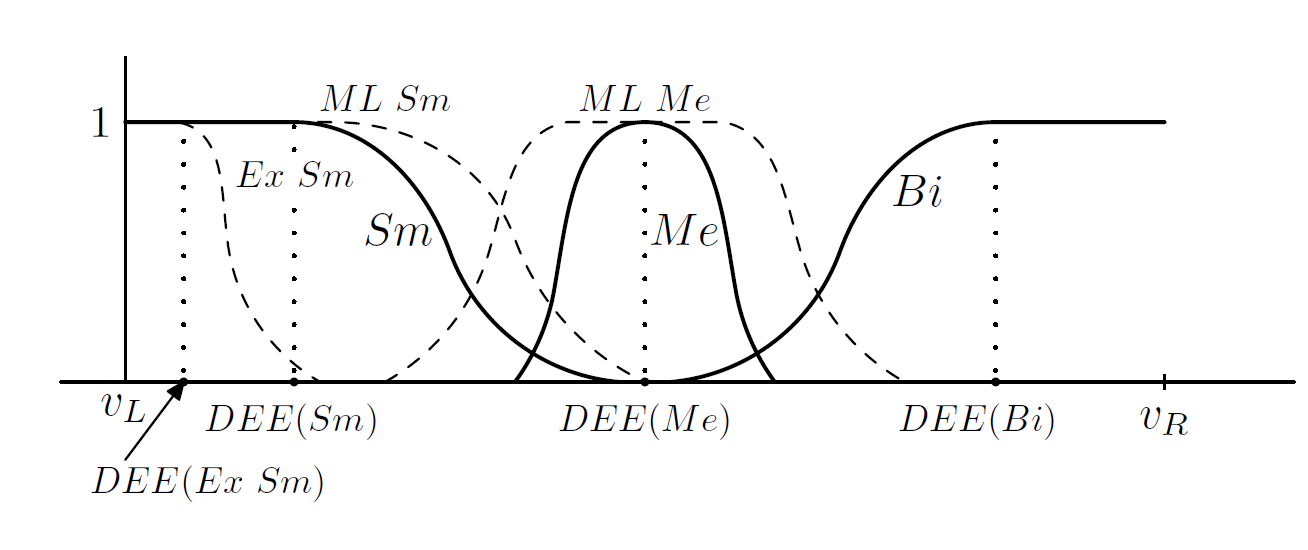
\includegraphics[scale=0.3]{DEE.png}
	\caption{Visual sketch of fuzzy sets representing some particular evaluative linguistic expressions. Specific defuzzification DEE is charted too.}\label{fig_dee}
\end{figure}

The ordering of hedges has an important role in the inference mechanism tailored to the linguistic fuzzy rules with the above mentioned evaluative linguistic expressions. It is based on specificity that is directly determined by the used hedge, assuming the same atomic expression is used. The  narrower the hedge, the more specific the expression is. And if an expression is more specific that another one, the respective fuzzy set that models its meaning is a fuzzy subset of the fuzzy set that models the less specific expression. This inclusion is visualized on Fig.~\ref{fig_dee}.



\subsection{Linguistic context}
\label{sec:context}

The \emph{linguistic context} is a sort of extended notion to the notion of the universe in a sense that the universe is also accompanied with some fundamental points. For the case of modeling expressions on numerical axis, we may dare to restrict our focus to universes that are closed real intervals so, the universe would be $U = [v_L, v_R]$. In order to talk about linguistic expression, we need to add at least the third ``middle'' point that does not represent the center of the interval however, it denotes the most typical value for middle size objects in the given domain. Usually, as humans are more sensitive to smaller values than to the big ones, the middle point is closer to $v_L$ than to $v_R$. For example, we may consider the universe of pine trees $U=[3,80]$ (in meters) while the middle size pine tree would be rather around 15-20 meters than in the middle of the interval $U$. So, extending the context to $[v_L, v_C, v_R]$ is not just a redundant adding of the central point $v_C$ but a desirable specification of the prototypical middle point $v_C$. 

As the context has to reflect \emph{unilateral/bilateral} nature (if it respects the positive and negative values) or the decision whether we deal with \emph{trichotomy} or a \emph{pentachotomy} (pentachotomy would require two more such emphasized points), the order triplet $[v_L, v_C, v_R]$ is not the only choice but the most fundamental and the simplest form of a linguistic context. In particular,  four different contexts are supported in \pkg{lfl}, and the above-mentioned simplest context is the \emph{unilateral trichotomy} that is chosen by calling the function \code{ctx3()}. The higher density of atomic expressions can be obtained by adding expressions \emph{``lower middle''} and \emph{``upper middle''}, which requires to consider \emph{unilateral pentachotomy} by calling the function \code{ctx5()}. The bilateral versions of the trichotomy and the pentachotomy allow to deal with expressions such as \emph{``negative small''}, \emph{``positive medium''}, or \emph{``negative very small''} and can be called by functions  \code{ctx3bilat()} and \code{ctx5bilat()}, respectively. The summary of functions responsible for creation of the linguistic context is provided below:
%
\begin{itemize}
    \item \code{ctx3(low, center, high)}: the unilateral trichotomy that enables the atomic expressions: \emph{``small'', ``medium'', ``big''}; 
    \item \code{ctx5(low, lowerCenter, center, upperCenter, high)} -- the unilateral pentacho\-to\-my that enables the atomic expressions: \emph{``small'', ``lower medium'', ``medium'', ``upper medium'', ``big''}; 
    \item \code{ctx3bilat(negMax, negCenter, origin, center, max)} -- the bilateral trichotomy that enables the atomic expressions: \emph{``negative big'', ``negative medium'', ``negative small'', ``zero'', ``small'', ``medium'', ``big''};
    \item \code{ctx5bilat(negMax, negUpperCenter, negCenter, negLowerCenter, origin, low\-erCenter, center, upperCenter, max)} -- the bilateral pentachotomy that enables the atomic expressions: \emph{``negative big'', ``negative upper medium'', ``negative medium'', ``negative lower medium'', ``negative small'', ``zero'', ``small'', ``lower medium'', ``medium'', ``upper medium'', ``big''}.
\end{itemize}
%
The arguments of context creator functions have sensible defaults and need not be therefore explicitly stated in all cases:
%
\begin{Schunk}
% --begin: "ctx"
\begin{Sinput}
R> ctx3(5, 100, 1000)
\end{Sinput}
\begin{Soutput}
Linguistic context: unilateral trichotomy (ctx3)
   low center   high 
     5    100   1000 
\end{Soutput}
\begin{Sinput}
R> ctx3()
\end{Sinput}
\begin{Soutput}
Linguistic context: unilateral trichotomy (ctx3)
   low center   high 
   0.0    0.5    1.0 
\end{Soutput}
\begin{Sinput}
R> ctx3(high = 100)
\end{Sinput}
\begin{Soutput}
Linguistic context: unilateral trichotomy (ctx3)
   low center   high 
     0     50    100 
\end{Soutput}
\begin{Sinput}
R> ctx5bilat()
\end{Sinput}
\begin{Soutput}
Linguistic context: bilateral pentachotomy (ctx5bilat)
        negMax negUpperCenter      negCenter negLowerCenter 
         -1.00          -0.75          -0.50          -0.25 
        origin    lowerCenter         center    upperCenter 
          0.00           0.25           0.50           0.75 
           max 
          1.00 
\end{Soutput}
\begin{Sinput}
R> ctx5bilat(negMax = -100, max = 200)
\end{Sinput}
\begin{Soutput}
Linguistic context: bilateral pentachotomy (ctx5bilat)
        negMax negUpperCenter      negCenter negLowerCenter 
          -100            -75            -50            -25 
        origin    lowerCenter         center    upperCenter 
             0             50            100            150 
           max 
           200 
\end{Soutput}
%
% --end: "ctx"
\end{Schunk}

%
Alternatively, the context may be automatically determined from data by calling the \code{minmax()} function, which creates the selected type of the context based on the minimum and maximum value found in data:
%
\begin{Schunk}
% --begin: "minmax"
\begin{Sinput}
data <- runif(n = 100, min = 20, max = 5000)
summary(data)
\end{Sinput}
\begin{Soutput}
##    Min. 1st Qu.  Median    Mean 3rd Qu.    Max. 
##   118.6  1306.3  2539.8  2580.3  3794.6  4997.8
\end{Soutput}
\begin{Sinput}
minmax(data, type = "ctx3")
\end{Sinput}
\begin{Soutput}
## Linguistic context: unilateral trichotomy (ctx3)
##      low   center     high 
##  118.573 2558.195 4997.816
\end{Soutput}
%
% --end: "minmax"
\end{Schunk}

%
The \code{minmax()} function may be forced not to guess some values by specifying them explicitly as additional arguments:
%
\begin{Schunk}
% --begin: "minmax2"
\begin{Sinput}
 minmax(data, type = "ctx3", center = 1000)
\end{Sinput}
\begin{Soutput}
Linguistic context: unilateral trichotomy (ctx3)
     low   center     high 
 118.573 1000.000 4997.816 
\end{Soutput}
%
% --end: "minmax2"
\end{Schunk}




\subsection{Evaluative linguistic expressions}
\label{sec:evallingexp}

The atomic expressions, e.g., \emph{``small''}, \emph{``medium''} or \emph{``big''} in the case of the unilateral trichotomy, are according to the theory of evaluative linguistic expressions \citep{Novak08} modelled with help of the \code{horizon()} function. Horizon of the atomic expression is a function that represents basic limits of what humans treat as small, medium or big, see Fig.~\ref{fig:horizon}.
%
\begin{Schunk}
% --begin: "horizon"
\begin{Sinput}
ctx <- ctx3()
smHoriz <- horizon(ctx, atomic = "sm")
smHoriz(seq(from = 0, to = 1, by = 0.2))
\end{Sinput}
\begin{Soutput}
## [1] 1.0 0.6 0.2 0.0 0.0 0.0
\end{Soutput}
%
% --end: "horizon"
\end{Schunk}

%

\begin{figure}
    \centering
    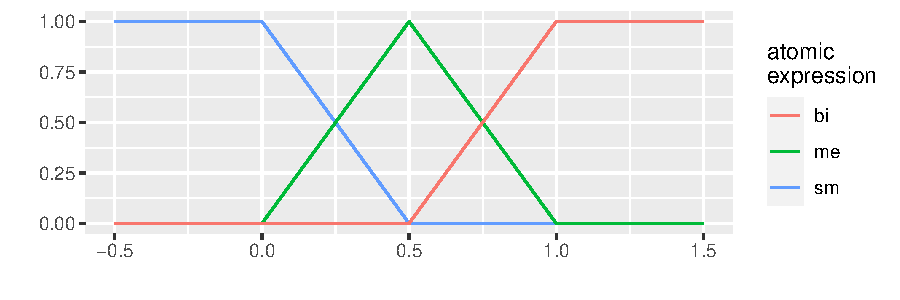
\includegraphics[scale=0.8]{figure/horizon-1.pdf}
    \caption{Horizons for the atomic expressions \emph{small}, \emph{medium} and \emph{big} in the unilateral trichotomy (\code{ctx3(0, 0.5, 1)})}
    \label{fig:horizon}
\end{figure}

A particular linguistic expression is obtained after the application of the linguistic hedge. So, in \pkg{lfl}, the \code{hedge()} function works as a modifier function, which is applied to a particular horizon. For instance, the function that represents the ``very small'' expression can be obtained as follows:
%
\begin{Schunk}
% --begin: "hedge"
\begin{Sinput}
R> veHedge <- hedge("ve")
R> ve.sm <- function(x) veHedge(smHoriz(x))
R> ve.sm(seq(from = 0, to = 0.5, by = 0.1))
\end{Sinput}
\begin{Soutput}
[1] 1.000000 0.585098 0.000000 0.000000 0.000000 0.000000
\end{Soutput}
%
% --end: "hedge"
\end{Schunk}

%
Such an approach gives the user a detailed control of the creation of a linguistic expression, which may be useful for experimenting with novel expressions. However, it may be tedious to manually create the functions for a routine use. Therefore, the \code{lingexpr()} function provides a shortcut for creation of pre-defined expressions:
%
\begin{Schunk}
% --begin: "lingexpr"
\begin{Sinput}
ve.sm2 <- lingexpr(ctx, atomic="sm", hedge="ve")
ve.sm2(seq(from=0, to=0.5, by=0.1))
\end{Sinput}
\begin{Soutput}
## [1] 1.000000 0.585098 0.000000 0.000000 0.000000 0.000000
\end{Soutput}
%
% --end: "lingexpr"
\end{Schunk}


An expression, consisting of an atomic expression only, is constructed using an empty hedge:
%
\begin{Schunk}
% --begin: "emptyhedge1"
\begin{Sinput}
emptyHedge <- hedge("-")
sm <- function(x) emptyHedge(smHoriz(x))
sm(seq(from = 0, to = 0.5, by = 0.1))
\end{Sinput}
\begin{Soutput}
## [1] 1.0000000 0.9620685 0.2439553 0.0000000 0.0000000 0.0000000
\end{Soutput}
%
% --end: "emptyhedge1"
\end{Schunk}

%
or equivalently:
%
\begin{Schunk}
% --begin: "emptyhedge2"
\begin{Sinput}
R> sm2 <- lingexpr(ctx, atomic = "sm", hedge = "-")
R> sm2(seq(from = 0, to = 0.5, by = 0.1))
\end{Sinput}
\begin{Soutput}
[1] 1.0000000 0.9620685 0.2439553 0.0000000 0.0000000 0.0000000
\end{Soutput}
%
% --end: "emptyhedge2"
\end{Schunk}

%
Figure~\ref{fig:lingexpr} shows all linguistic expressions of the unilateral trichotomy context (\code{ctx3}).

\begin{figure}[h]
    \centering
    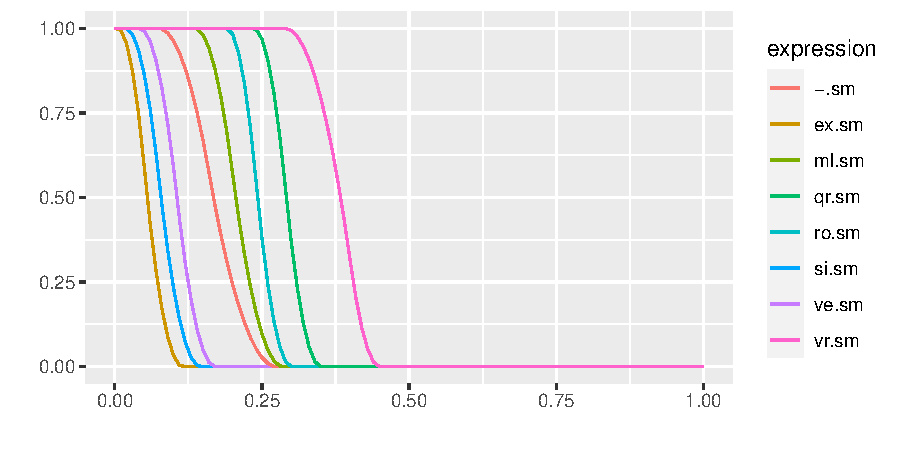
\includegraphics[scale=0.59]{figure/lingexpr1-1.pdf}
    \\
    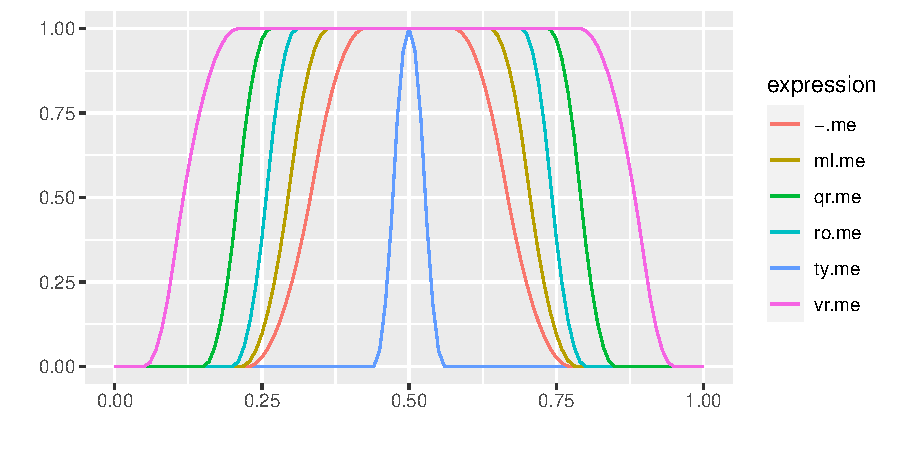
\includegraphics[scale=0.59]{figure/lingexpr2-1.pdf}
    \\
    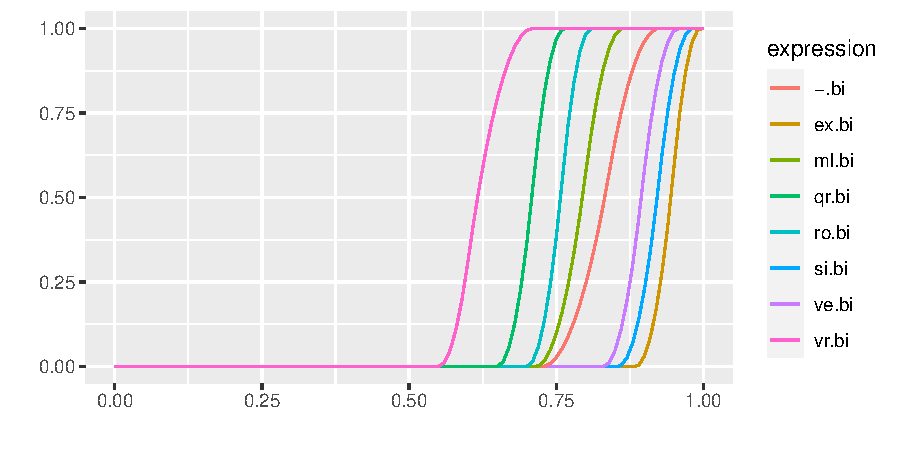
\includegraphics[scale=0.59]{figure/lingexpr3-1.pdf}
    \caption{All pre-defined linguistic expressions for the unilateral trichotomy context \code{ctx3}}
    \label{fig:lingexpr}
\end{figure}


   

\subsection{Other functions}

For the sake of completeness, the \pkg{lfl} package provides tools for the creation of triangular or raised-cosine functions. Both \code{triangular()} and \code{raisedcosine()} functions take three arguments, \code{lo}, \code{center}, \code{hi}, which fully parameterize the shape of the resulting function. See the example below as well as Figure~\ref{fig:triangular} for more detail. Note also that the \code{lo} and \code{hi} parameters may be set to an infinite value (\code{-Inf} resp. \code{Inf}), which causes the particular tail to be constantly equal to 1.
%
\begin{Schunk}
% --begin: "triangular"
\begin{Sinput}
tri <- triangular(0, 0.5, 1)
tri(seq(from = 0, to = 1, by = 0.2))
\end{Sinput}
\begin{Soutput}
## [1] 0.0 0.4 0.8 0.8 0.4 0.0
\end{Soutput}
\begin{Sinput}
rcos <- raisedcosine(0, 0.5, 1)
rcos(seq(from = 0, to = 1, by = 0.2))
\end{Sinput}
\begin{Soutput}
## [1] 0.0000000 0.3454915 0.9045085 0.9045085 0.3454915 0.0000000
\end{Soutput}
%
% --end: "triangular"
\end{Schunk}


\begin{figure}[h]
    \centering
    \begin{subfigure}[b]{0.49\textwidth}
        \centering
        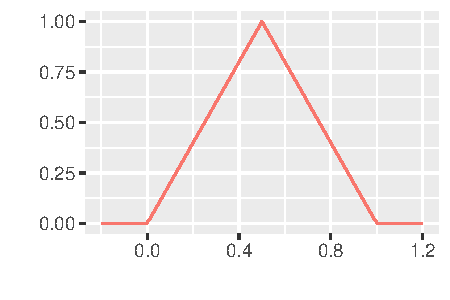
\includegraphics[scale=0.80]{figure/triangular1-1.pdf}
        \caption{\code{triangular(0, 0.5, 1)}}
    \end{subfigure}
    \begin{subfigure}[b]{0.49\textwidth}
        \centering
        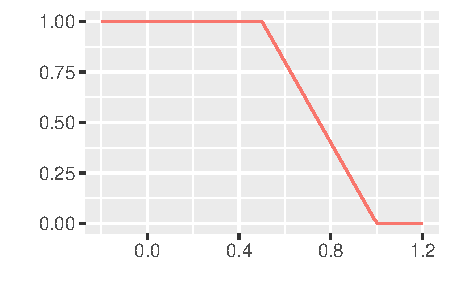
\includegraphics[scale=0.80]{figure/triangular2-1.pdf}
        \caption{\code{triangular(-Inf, 0.5, 1)}}
    \end{subfigure}
    \begin{subfigure}[b]{0.49\textwidth}
        \centering
        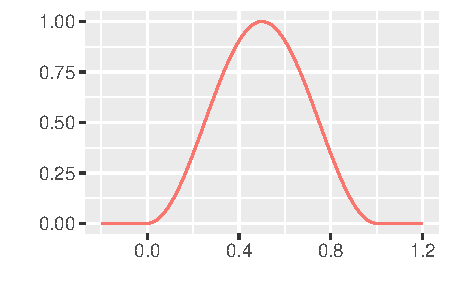
\includegraphics[scale=0.80]{figure/raisedcos1-1.pdf}
        \caption{\code{raisedcosinal(0, 0.5, 1)}}
    \end{subfigure}
    \begin{subfigure}[b]{0.49\textwidth}
        \centering
        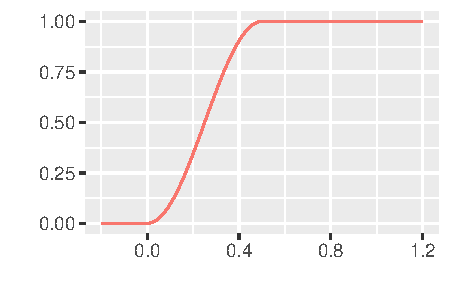
\includegraphics[scale=0.80]{figure/raisedcos2-1.pdf}
        \caption{\code{raisedcosinal(0, 0.5, Inf)}}
    \end{subfigure}
    \caption{Triangular and raised-cosinal functions}
    \label{fig:triangular}
\end{figure}


\subsection{Batch transformations of data to membership degrees of fuzzy sets}
\label{sec:lcut}

Practical applications often require to transform data into multiple fuzzy sets. The \pkg{lfl} package provides the \code{lcut()} and \code{fcut()} functions to perform such transformations. Both functions transform vectors (numeric, logical or factors), matrices or data frames into an \code{fsets} object. Such an object is a data frame with each column representing a single fuzzy set. The values are from the $[0, 1]$ interval and they are equal to the membership degrees of the element of the universe to the particular fuzzy sets. These functions are the fuzzy-counterparts of the well known \code{cut()} operation of the base \R{}.

For logical input, the \code{lcut()} function returns two columns of 0s and 1s: these columns represent (crisp) truth degrees equivalent to the original input and its negation, respectively. The name of the column is either specified by the user in the \code{name} argument, or derived from the given data argument automatically:
%
\begin{Schunk}
% --begin: "lcut.logical"
\begin{Sinput}
logvec <- c(TRUE, FALSE, TRUE, TRUE)
lcut(logvec)
\end{Sinput}
\begin{Soutput}
##      logvec not.logvec
## [1,]      1          0
## [2,]      0          1
## [3,]      1          0
## [4,]      1          0
\end{Soutput}
\begin{Sinput}
lcut(logvec, name = "employed")
\end{Sinput}
\begin{Soutput}
##      employed not.employed
## [1,]        1            0
## [2,]        0            1
## [3,]        1            0
## [4,]        1            0
\end{Soutput}
%
% --end: "lcut.logical"
\end{Schunk}

%
The factor input is dichotomized in the result:
%
\begin{Schunk}
% --begin: "lcut.factor"
\begin{Sinput}
 position <- factor(c("worker", "manager", "worker", "accountant"))
 lcut(position)
\end{Sinput}
\begin{Soutput}
     position=accountant position=manager position=worker
[1,]                   0                0               1
[2,]                   0                1               0
[3,]                   0                0               1
[4,]                   1                0               0
\end{Soutput}
%
% --end: "lcut.factor"
\end{Schunk}


For numeric input, the \code{lcut()} function performs transformation to linguistic expressions similarly as described in Section~\ref{sec:evallingexp}. For this step, a linguistic context must be provided (see Section~\ref{sec:context}). If the context is not provided, it is determined automatically using the \code{minmax()} function described in Section~\ref{sec:context}. The required atomic expressions or hedges may be specified manually or leaved empty to let the system use all relevant combinations:
%
\begin{Schunk}
% --begin: "lcut.numeric"
\begin{Sinput}
R> age <- round(runif(n = 5, min = 18, max = 65))
R> print(age)
\end{Sinput}
\begin{Soutput}
[1] 55 32 41 52 51
\end{Soutput}
\begin{Sinput}
R> lcut(age, context = ctx3(low = 0, high = 100))
\end{Sinput}
\begin{Soutput}
     ex.sm.age si.sm.age ve.sm.age sm.age ml.sm.age ro.sm.age
[1,]         0         0         0      0         0         0
[2,]         0         0         0      0         0         0
[3,]         0         0         0      0         0         0
[4,]         0         0         0      0         0         0
[5,]         0         0         0      0         0         0
     qr.sm.age vr.sm.age  ty.me.age    me.age ml.me.age
[1,] 0.0000000 0.0000000 0.04761905 1.0000000 1.0000000
[2,] 0.1315789 0.9475480 0.00000000 0.3914128 0.7993319
[3,] 0.0000000 0.1993769 0.00000000 0.9859853 1.0000000
[4,] 0.0000000 0.0000000 0.73333333 1.0000000 1.0000000
[5,] 0.0000000 0.0000000 0.93333333 1.0000000 1.0000000
     ro.me.age qr.me.age vr.me.age ex.bi.age si.bi.age ve.bi.age
[1,]         1         1         1         0         0         0
[2,]         1         1         1         0         0         0
[3,]         1         1         1         0         0         0
[4,]         1         1         1         0         0         0
[5,]         1         1         1         0         0         0
     bi.age ml.bi.age ro.bi.age qr.bi.age vr.bi.age
[1,]      0         0         0         0         0
[2,]      0         0         0         0         0
[3,]      0         0         0         0         0
[4,]      0         0         0         0         0
[5,]      0         0         0         0         0
\end{Soutput}
%
% --end: "lcut.numeric"
\end{Schunk}


If data frame is to be processed with the \code{lcut()} function, the result is created per column. Also note that the names of the resulting variables are derived from the column names of the input data frame:
%
\begin{Schunk}
% --begin: "lcut.data.frame"
\begin{Sinput}
R> data <- data.frame(position=position,
+                     age=age,
+                     employed=logvec)
R> print(data)
\end{Sinput}
\begin{Soutput}
    position age employed
1     worker  55     TRUE
2    manager  32    FALSE
3     worker  41    FALSE
4     worker  52     TRUE
5 accountant  51     TRUE
\end{Soutput}
\begin{Sinput}
R> employees <- lcut(data,
+       context=ctx3(low=0, high=100),
+       atomic=c("sm", "me", "bi"),
+       hedges=c("ve", "-", "ro"))
R> print(employees)
\end{Sinput}
\begin{Soutput}
     position=accountant position=manager position=worker
[1,]                   0                0               1
[2,]                   0                1               0
[3,]                   0                0               1
[4,]                   0                0               1
[5,]                   1                0               0
     ve.sm.age sm.age ro.sm.age    me.age ro.me.age ve.bi.age
[1,]         0      0         0 1.0000000         1         0
[2,]         0      0         0 0.3914128         1         0
[3,]         0      0         0 0.9859853         1         0
[4,]         0      0         0 1.0000000         1         0
[5,]         0      0         0 1.0000000         1         0
     bi.age ro.bi.age employed not.employed
[1,]      0         0        1            0
[2,]      0         0        0            1
[3,]      0         0        0            1
[4,]      0         0        1            0
[5,]      0         0        1            0
\end{Soutput}
%
% --end: "lcut.data.frame"
\end{Schunk}

%
The given contexts, atomic expressions and hedges are recycled for each input numeric column. If a different setting is needed for each column, the arguments should be given as named lists as follows:
%
\begin{Schunk}
% --begin: "lcut.data.frame2"
\begin{Sinput}
data$salary <- round(runif(n=4, min=1000, max=20000))
print(data)
\end{Sinput}
\begin{Soutput}
##     position age employed salary
## 1     worker  55     TRUE  14191
## 2    manager  32    FALSE   7728
## 3     worker  41     TRUE  16279
## 4 accountant  52     TRUE  15044
\end{Soutput}
\begin{Sinput}
employees <- lcut(data,
                  context=list(age=ctx3(low=0, high=100),
                               salary=ctx3(low=500, high=50000)),
                  atomic=list(salary=c("sm", "bi")),
                  hedges=list(age=c("ve", "-", "ro"),
                              salary=c("ex", "ve", "-", "ro")))
print(colnames(employees))
\end{Sinput}
\begin{Soutput}
##  [1] "position=accountant" "position=manager"    "position=worker"    
##  [4] "ve.sm.age"           "sm.age"              "ro.sm.age"          
##  [7] "me.age"              "ro.me.age"           "ve.bi.age"          
## [10] "bi.age"              "ro.bi.age"           "employed"           
## [13] "not.employed"        "ex.sm.salary"        "ve.sm.salary"       
## [16] "sm.salary"           "ro.sm.salary"        "ex.bi.salary"       
## [19] "ve.bi.salary"        "bi.salary"           "ro.bi.salary"
\end{Soutput}
%
% --end: "lcut.data.frame2"
\end{Schunk}



The \code{fsets} object returned by the \code{lcut()} function (and the \code{fcut()} function as well, see below) handles an additional information, the \code{vars} and \code{specs} attributes. In particular, \code{vars} is a character vector that assigns the original data name to each of the resulting column of membership degrees. In other words, the \code{vars} vector specifies the equivalence classes of fuzzy sets that were originated from the same data:
%
\begin{Schunk}
% --begin: "lcut.vars"
\begin{Sinput}
vars(employees)
\end{Sinput}
\begin{Soutput}
##  [1] "position" "position" "position" "age"      "age"      "age"     
##  [7] "age"      "age"      "age"      "age"      "age"      "employed"
## [13] "employed" "salary"   "salary"   "salary"   "salary"   "salary"  
## [19] "salary"   "salary"   "salary"
\end{Soutput}
%
% --end: "lcut.vars"
\end{Schunk}

%
The \code{specs} attribute returns a matrix that encodes a sort of \emph{specificity} relation (see Section~\ref{sec:pbld}) between the columns of the \code{fsets} object. (In the following example, some columns and rows are omitted for brevity.
%
\begin{Schunk}
% --begin: "lcut.specs"
\begin{Sinput}
specs(employees)[1:5, 1:5]
\end{Sinput}
\begin{Soutput}
##      [,1] [,2] [,3] [,4] [,5]
## [1,]    0    0    0    0    0
## [2,]    0    0    0    0    0
## [3,]    0    0    0    0    0
## [4,]    0    0    0    0    1
## [5,]    0    0    0    0    0
\end{Soutput}
%
% --end: "lcut.specs"
\end{Schunk}

%
As can be seen, the 4th fuzzy set (\code{ve.sm.age}) is more specific than 5th (\code{sm.age}), which is more specific than the 6th fuzzy set (\code{ro.sm.age}).


The \code{fcut()} function works identically to \code{lcut()} for logical and factor input:
%
\begin{Schunk}
% --begin: "fcut.logfact"
\begin{Sinput}
R> logvec <- c(TRUE, FALSE, FALSE, TRUE, TRUE)
R> position <- factor(c("worker", "manager", "worker", "worker", "accountant"))
R> fcut(data.frame(employed = logvec, position = position))
\end{Sinput}
\begin{Soutput}
     employed not.employed position=accountant position=manager
[1,]        1            0                   0                0
[2,]        0            1                   0                1
[3,]        0            1                   0                0
[4,]        1            0                   0                0
[5,]        1            0                   1                0
     position=worker
[1,]               1
[2,]               0
[3,]               1
[4,]               1
[5,]               0
\end{Soutput}
%
% --end: "fcut.logfact"
\end{Schunk}

%
Numerical values are transformed with the \code{fcut()} function to triangular or raised-cosine membership degrees (depending on the \code{type} argument which has to be either \code{"triangle"} or \code{"raisedcos"}):
%
\begin{Schunk}
% --begin: "fcut.numeric1"
\begin{Sinput}
R> numvec <- 1:9
R> fcut(numvec,
+       breaks=c(1, 5, 9),
+       type="triangle")
\end{Sinput}
\begin{Soutput}
      numvec=1
 [1,]     0.00
 [2,]     0.25
 [3,]     0.50
 [4,]     0.75
 [5,]     1.00
 [6,]     0.75
 [7,]     0.50
 [8,]     0.25
 [9,]     0.00
\end{Soutput}
%
% --end: "fcut.numeric1"
\end{Schunk}

%
The preceding example is identical to the call of the \code{triangular()} function:
%
\begin{Schunk}
% --begin: "fcut.triangular"
\begin{Sinput}
 triangular(1, 5, 9)(numvec)
\end{Sinput}
\begin{Soutput}
[1] 0.00 0.25 0.50 0.75 1.00 0.75 0.50 0.25 0.00
\end{Soutput}
%
% --end: "fcut.triangular"
\end{Schunk}

%

However, the \code{fcut()} function is mainly useful for creation of multiple fuzzy sets. A mandatory \code{breaks} argument determines the break-points of the positions of the fuzzy sets. It should be an ordered vector of numbers such that the $i$-th index specifies the infimum of the support (left-hand side corner), $(i+1)$-th the center, and $(i+2)$-th the supremum of the support of the $i$-th fuzzy set. The minimum number of breaks-points is 3. $n-2$ elementary fuzzy sets would be created for $n$ break-points.

For instance, the following command produces three triangular fuzzy sets with parameters $(1, 3, 5)$, $(3, 5, 7)$ and $(5, 7, 9)$:
%
\begin{Schunk}
% --begin: "fcut.numeric2"
\begin{Sinput}
R> fcut(numvec, breaks = c(1, 3, 5, 7, 9), type = "triangle")
\end{Sinput}
\begin{Soutput}
      numvec=1 numvec=2 numvec=3
 [1,]      0.0      0.0      0.0
 [2,]      0.5      0.0      0.0
 [3,]      1.0      0.0      0.0
 [4,]      0.5      0.5      0.0
 [5,]      0.0      1.0      0.0
 [6,]      0.0      0.5      0.5
 [7,]      0.0      0.0      1.0
 [8,]      0.0      0.0      0.5
 [9,]      0.0      0.0      0.0
\end{Soutput}
%
% --end: "fcut.numeric2"
\end{Schunk}

%

Let us consider the $i$-th fuzzy set. The values smaller than the $i$-th break and greater than $(i+2)$-th break result in the zero membership degree, values equal to $(i+1)$-th break result in the membership degree equal 1, and values between them result in a membership degree between 0 and 1 accordingly to the specified \code{type} (\code{"triangle"} or \code{"raisedcos"}).
Names of resulting fuzzy sets are created from the name of the original data variable (\code{numvec} in this case), the symbol of equality (\code{=}) and a number $i$.

\begin{figure}[h]
    \centering
    \newsavebox{\largestimage}
    \savebox{\largestimage}{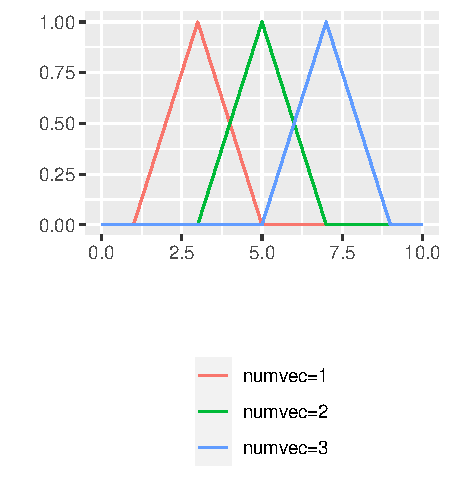
\includegraphics[width=0.4\textwidth]{figure/fcut_plot1-1.pdf}}
    \begin{subfigure}[b]{0.49\textwidth}
        \centering
        \usebox{\largestimage}
        \caption{\code{merge=1}}
    \end{subfigure}
    \begin{subfigure}[b]{0.49\textwidth}
        \centering
        \raisebox{\dimexpr0.07\ht\largestimage}{%
            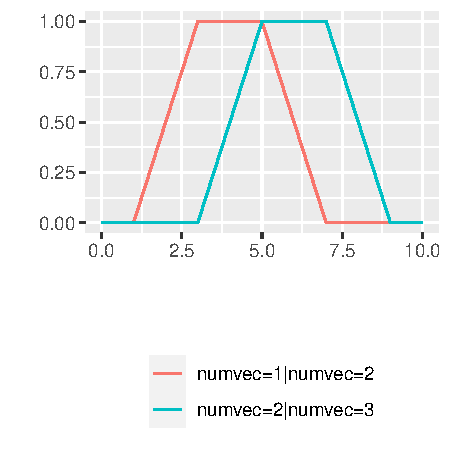
\includegraphics[width=0.82\textwidth]{figure/fcut_plot2-1.pdf}}
        \caption{\code{merge=2}}
    \end{subfigure}
    \caption{Results of the \code{fcut} call with \code{breaks=c(1, 3, 5, 7, 9)} and different settings of \code{merge}.}
    \label{fig:fcut}
\end{figure}



Additionally, combined fuzzy sets may be created by using the argument \code{merge}. If \code{merge=1} (the default), only the elementary fuzzy sets discussed above are produced. 
Setting \code{merge=2} means that each two consecutive elementary fuzzy sets should be combined with the \L{}ukasiewicz t-conorm into a single fuzzy set, \code{merge=3} causes combining three consecutive elementary fuzzy sets etc. See Fig.~\ref{fig:fcut} and also the following example.


The \code{merge} argument determines whether to derive additional fuzzy sets by merging the elementary fuzzy sets (defined with the \code{breaks} argument) into super-sets. The \code{merge} may contain any integer number from \code{1} to \code{length(breaks) - 2}. Value \code{1} means that the elementary fuzzy sets have to be created only, as described above (the default case). 

%
\begin{Schunk}
% --begin: "fcut.merge"
\begin{Sinput}
R> fcut(numvec,
+       breaks=c(1, 3, 5, 7, 9),
+       merge=2,
+       type="triangle")
\end{Sinput}
\begin{Soutput}
      numvec=1|numvec=2 numvec=2|numvec=3
 [1,]               0.0               0.0
 [2,]               0.5               0.0
 [3,]               1.0               0.0
 [4,]               1.0               0.5
 [5,]               1.0               1.0
 [6,]               0.5               1.0
 [7,]               0.0               1.0
 [8,]               0.0               0.5
 [9,]               0.0               0.0
\end{Soutput}
\begin{Sinput}
R> fcut(numvec,
+       breaks=c(1, 3, 5, 7, 9),
+       merge=3,
+       type="triangle")
\end{Sinput}
\begin{Soutput}
      numvec=1|numvec=2|numvec=3
 [1,]                        0.0
 [2,]                        0.5
 [3,]                        1.0
 [4,]                        1.0
 [5,]                        1.0
 [6,]                        1.0
 [7,]                        1.0
 [8,]                        0.5
 [9,]                        0.0
\end{Soutput}
%
% --end: "fcut.merge"
\end{Schunk}

%



The \code{merge} argument may contain multiple values. In that case, all types of merged fuzzy sets are provided. In the following example, the \code{merge} argument is a numeric vector containing \code{1, 2, 3}, which means that the elementary fuzzy sets are created (\code{1}), the combinations of two consecutive elementary fuzzy sets are provided too (\code{2}), as also a single fuzzy set that combines all the three elementary fuzzy sets is returned (\code{3}):
%
\begin{Schunk}
% --begin: "fcut.merge2"
\begin{Sinput}
 fd <- fcut(numvec, breaks = c(1, 3, 5, 7, 9), merge = c(1, 2, 3), type = "triangle")
 print(colnames(fd))
\end{Sinput}
\begin{Soutput}
[1] "numvec=1"                   "numvec=2"                  
[3] "numvec=3"                   "numvec=1|numvec=2"         
[5] "numvec=2|numvec=3"          "numvec=1|numvec=2|numvec=3"
\end{Soutput}
%
% --end: "fcut.merge2"
\end{Schunk}

%
As can be seen, the names of the derived (merged) fuzzy sets are created from the names of the original elementary fuzzy sets by concatenating them with the pipe (\code{|}) separator. 

Similarly as for \code{lcut()}, the result of the \code{fcut()} function is an instance of the \code{fsets} object. Hence the additional information, the \code{vars} and \code{specs} attributes discussed above, is also available:
%
\begin{Schunk}
% --begin: "fcut.varsspecs"
\begin{Sinput}
vars(fd)
\end{Sinput}
\begin{Soutput}
## [1] "numvec" "numvec" "numvec" "numvec" "numvec" "numvec"
\end{Soutput}
\begin{Sinput}
specs(fd)
\end{Sinput}
\begin{Soutput}
##      [,1] [,2] [,3] [,4] [,5] [,6]
## [1,]    0    0    0    1    0    1
## [2,]    0    0    0    1    1    1
## [3,]    0    0    0    0    1    1
## [4,]    0    0    0    0    0    1
## [5,]    0    0    0    0    0    1
## [6,]    0    0    0    0    0    0
\end{Soutput}
%
% --end: "fcut.varsspecs"
\end{Schunk}

%


%\subsection{Linguistic expressions in generalized quantifiers}
%\label{sec:fuz_quant}





%The evaluative linguistic expressions may be directly used in the construction of the predefined quantifiers. Indeed, let us consider the $\langle 1, 1\rangle$ quantifiers as defined by \cite{murinova2020}. We recall that the \code{w} argument must be set to truth values of the antecedent, e.g., ``at least five \code{B}s are \code{A}'' may be evaluated by:
%
%\begin{Schunk}
% --begin: "quant4"
\begin{Sinput}
R> atLeast5(lukas.residuum(B, A), w = B)
\end{Sinput}
\begin{Soutput}
[1] 1.0 1.0 1.0 1.0 0.8 0.0
[1] 0 0 0 0 0 1
\end{Soutput}
\begin{Soutput}
[1] 0
\end{Soutput}
%
% --end: "quant4"
\end{Schunk}

%


%The used relative measures may be derived from evaluative linguistic expressions discussed in Section~\ref{sec:lingexpr}. Pre-defined quantifiers may be created by calling the \code{quantifier()} function, which is a wrapper over \code{quant()}:
%
%\begin{Schunk}
% --begin: "quant5"
\begin{Sinput}
 almost <- quantifier("almost.all")
 most <- quantifier("most")
 many <- quantifier("many")
 almost(A)
\end{Sinput}
\begin{Soutput}
[1] 0
\end{Soutput}
\begin{Sinput}
 most(A)
\end{Sinput}
\begin{Soutput}
[1] 0.001340707
\end{Soutput}
\begin{Sinput}
 many(A)
\end{Sinput}
\begin{Soutput}
[1] 1
\end{Soutput}
%
% --end: "quant5"
\end{Schunk}

%





\section{Fuzzy association rules}
\label{sec:assoc}

\subsection{Theoretical background}

The association rules \citep{Agrawal:assoc_rules} need not be introduced in detail, we only recall the fact that firstly the method appeared under the name GUHA \citep{Hajek:GUHA,HajekHavranek_GUHA} and furthermore, we recall basic principles of how this method finds  distinct statistically
approved associations between attributes of given objects. With help of \pkg{lfl} the method can be used also in the fuzzy setting, i.e., for graded properties. 


The crisp version of association rules deals with
Table~\ref{Tab:guha_exampleI} where $o_1,\dots, o_n$ denote objects,
$X_1,\dots , X_m$ denote independent boolean attributes, $Y_1,
\dots, Y_q$ denote the dependent boolean attributes, and
finally, symbols $a_{ij}$ and $b_{ij}$ are values from $ \{ 0,1 \}$ that denote
whether the $i$-th object $o_i$ carries attribute $X_j$ or $Y_j$, respectively. Each object can be represented as a boolean vector with $m+q$ components.

\begin{table}[ht]
  \centering
\begin{tabular}{|l|ccc|ccr|}
    \hline
          & $X_1$ & $\ldots$ & $X_m$ & $Y_1$ &  $\ldots$ & $Y_q$\\
    \hline
    $o_1$ & $a_{11}$ & $\ldots$ & $a_{1m}$ & $b_{11}$ &  $\ldots$ & $b_{1q}$\\
    $\vdots$ & $\vdots$ & $\ddots$ & $\vdots$ & $\vdots$ & $\ddots$ & $\vdots$\\
    $o_n$ & $a_{n1}$ & $\ldots$ & $a_{nm}$ & $b_{n1}$ &  $\ldots$ & $b_{nq}$\\
    \hline
\end{tabular}\caption{The table objects and attributes.} \label{Tab:guha_exampleI}
\end{table}

As the GUHA method deals with boolean attributes and features are often taking values from a real universe, the attributes are usually partitioned to intervals. Then the method seeks for associations:\begin{equation} {\tt A}(X_{i1},\ldots,X_{ip})\simeq
{\tt B}(Y_k) \label{form:assoc_general}
\end{equation}
where ${\tt A}$ is a predicate with conjunctively connected variables $X_{i1},\ldots,
X_{ip}$ (for $p\leq m$), and ${\tt
B}$ is a predicate with variables $Y_k$, for $k$ taking values from 1 to $q$. In order to mine such associations, a four-fold 
Table~\ref{Tab:4fold-guha} is constructed.
\begin{table}[ht]
\centering
\begin{tabular}{|r|lc|}
\hline
  & ${\tt B}$ & $\text{not}\; {\tt B}$ \\
    \hline
    ${\tt A}$ & $a$ & $b$\\
    $\text{not}\; {\tt A}$ & $c$ & $d$\\
    \hline
\end{tabular}
\caption{Four-fold table for mining linguistic associations.} \label{Tab:4fold-guha}
\end{table}



The number of synchronous occurrences of ${\tt A}$ and ${\tt B}$ is denoted by $a$ in Table~\ref{Tab:4fold-guha}, $b$ denotes the number of occurrences of ${\tt A}$ while ${\tt
B}$ does not hold, numbers $c$ and $d$ are determined analogously. Often, only numbers $a$ and $b$ are important for distinct qualitative measures. For instance, the relationship between ${\tt A}$ and ${\tt B}$ may be obtained with help of the \emph{binary multitudinal quantifier} $\simeq\
:=\ \sqsubset^{\gamma}_{r}$ that confirms the association if:
$$\frac{a}{a+b}>\gamma \qquad \textrm{and} \qquad \frac{a}{n}>r,$$
where $\gamma \in [0,1]$ is a \emph{degree of confidence} and
$r\in[0,1]$ is a \emph{degree of support}.



In order to soften the binary character of the associations and the sensitivity to the  partitioning of the universes into intervals, distinct approaches to fuzzy associations were employed
\cite{Sudkamp:2005,Kupka:NNW2010,Glass:FSS2008}.
The \pkg{lfl} package adopts the approach published in \cite{StepBurda:FRBE_FSS} because  it directly uses the theory of evaluative
linguistic expressions. The attributes are not boolean anymore. Recalling the example from \cite{StepBurda:FRBE_FSS}, we may consider independent variables BMI (Body Mass Index) and Chol (cholesterol level), and the dependent variable BP (blood pressure) and the attributes such as $\mathrm{BMI}^{\mathrm{Ve Bi}}$,
$\mathrm{BP}^{\mathrm{Me}}$, $\mathrm{Chol}^{\mathrm{Si Bi}}$
etc. that are defined by the fuzzy sets modeling  the particular evaluative expressions. In such a way, the authors obtained Table~\ref{Tab:FuzzyGuhaComplete}  with membership degrees $a_{ij} \in [0,1]$.

\begin{table}[ht]
  \centering
\begin{tabular}{|l| c c c |c c c|}
    \hline
          & $\mathrm{BMI}^{\mathrm{Ex
Sm}}$ &  \ldots & $\mathrm{Chol}^{\mathrm{Ex Bi}}$ & $\mathrm{BP}^{\mathrm{Ex Sm}}$ & \ldots & $\mathrm{BP}^{\mathrm{Ex Bi}}$\\
    \hline
    $o_1$ & 0.5 & \ldots & 0 & 1 & \ldots & 0\\
    $o_2$ & 0.8 & \ldots & 0  & 0.4 & \ldots & 0\\
    $o_3$ & 0 &  \ldots & 0.1  & 0 & \ldots & 0.4\\
    $o_4$ & 0 &  \ldots & 0.4  & 0 & \ldots & 0.3\\
    $o_5$ & 0.6  & \ldots & 0  & 1 & \ldots & 0\\
    $\vdots$  & $\vdots$ & $\vdots$ & $\vdots$ & $\vdots$ & $\vdots$& $\vdots$\\
    $o_n$ & 0 & \ldots & 0  & 0.5 & \ldots & 0 \\
    \hline
\end{tabular}
\caption{An example of the table with fuzzy attributes for fuzzy associations mining, ref. \cite{StepBurda:FRBE_FSS}. } \label{Tab:FuzzyGuhaComplete}
\end{table}



Table~\ref{Tab:4fold-guha} is
constructed for the fuzzy case in the same way using the cardinality, i.e., values $a,b,c,d$ are summations of membership degrees. The conjunctive aggregations of the truth-values of 
${\tt A}$ and ${\tt B}$ 
were modeled by the minimum operation however, other t-norms \citep{KlementMesiarPap00} may be considered as well. So, if the membership degree of $o_i$ to ${\tt A}$ is
0.4 and its membership degree to ${\tt B}$ is 0.7, the value that
enters the summation equals to $\min\{ 0.4,0.7\} = 0.4$. If we sum up such values over all objects, we obtain the number $a$ in
Table~\ref{Tab:4fold-guha}. The other numbers are determined in an analogous way. 


The advantage of associations (\ref{form:assoc_general}) is that each of them can be interpreted as the fuzzy rule:
$$\mathcal{R}\defeq\IFRuleMore{X_{i1}}{\mathcal{A}_{i1}}{X_{ip}}{\mathcal{A}_{ip}}{Y_k}{\mathcal{B}_{ik}}$$ that may be used in the inference systems for approximate reasoning. 



\subsection[Searching for fuzzy association rules in lfl]{Searching for fuzzy association rules in \pkg{lfl}}

The \pkg{lfl} package provides the \code{searchrules()} function that implements an OPUS-inspired algorithm \citep{webb95opus} for searching for fuzzy association rules in data. The \code{searchrules()} function traverses through the data set transformed to fuzzy sets (see \code{lcut()} and \code{fcut()} functions in Section~\ref{sec:lcut}) and searches for all rules that satisfy certain restrictive conditions specified by the user:
%
\begin{Schunk}
% --begin: "searchrules"
\begin{Sinput}
 rb <- searchrules(employees,
                   lhs=seq_len(ncol(employees)),
                   rhs=seq_len(ncol(employees)),
                   minSupport=0.5,
                   minConfidence=0.8,
                   maxLength=3)
 print(rb)
\end{Sinput}
\begin{Soutput}
                              support lhsSupport rhsSupport confidence
position=worker => employed 0.5000000  0.5000000  0.7500000  1.0000000
 => ro.me.age               1.0000000  1.0000000  1.0000000  1.0000000
employed => me.age          0.7464963  0.7500000  0.8443495  0.9953284
me.age => employed          0.7464963  0.8443495  0.7500000  0.8841082
 => me.age                  0.8443495  1.0000000  0.8443495  0.8443495
\end{Soutput}
%
% --end: "searchrules"
\end{Schunk}


Besides the \code{fsets} data object (see Section~\ref{sec:lcut}), the \code{searchrules()} function accepts the following arguments:
\begin{itemize}
    \item \code{lhs} -- indices of data columns that may appear on the left-hand side of the rule (i.e., in the antecedent);
    \item \code{rhs} -- indices of data columns that may appear on the right-hand side of the rule (i.e., in the consequent);
    \item \code{tnorm} -- the t-norm that represents the conjunction of predicates in the antecedent (defaults to G\"odel minimum);
    \item \code{n} -- the maximum number of rules with greatest confidence to be found;
    \item \code{minSupport} -- the minimum support degree of a rule. Rules with support below that number are filtered out;
    \item \code{minConfidence} -- the minimum confidence degree of a rule. Rules with confidence below that number are filtered out;
    \item \code{maxConfidence} -- the maximum confidence threshold. After finding a rule that has confidence degree above the maxConfidence threshold, no other rule is resulted based on adding some additional attribute to its antecedent part. So, if \code{a => c} has confidence above the \code{maxConfidence} threshold, no more rules containing \code{a} in the antecedent and \code{c} in the consequent will be produced regardless of their interest measures;
    \item \code{maxLength} -- the maximum allowed length of the antecedent, i.e. maximal number of predicates that are allowed to appear on both sides of the rule. If negative, the maximum length of rules is unlimited.
    \item \code{numThreads} -- the number of computing threads to start in parallel multi-threaded computation.
\end{itemize}



Internally, the rule base produced by the \code{searchrules()} function is an instance of the \code{farules} class. It is a list of two elements, \code{rules} and \code{statistics}, where \code{rules} is a list of character vectors of rule predicate names. The first element of these vectors is a consequent of the rule, the rest is the antecedent. The \code{statistics} element is a matrix that assigns some quality measures to each rule:
%
\begin{Schunk}
% --begin: "searchrules2"
\begin{Sinput}
str(rb)
\end{Sinput}
\begin{Soutput}
## List of 2
##  $ rules     :List of 5
##   ..$ : chr [1:2] "employed" "position=worker"
##   ..$ : chr "ro.me.age"
##   ..$ : chr [1:2] "me.age" "employed"
##   ..$ : chr [1:2] "employed" "me.age"
##   ..$ : chr "me.age"
##  $ statistics: num [1:5, 1:4] 0.5 1 0.746 0.746 0.844 ...
##   ..- attr(*, "dimnames")=List of 2
##   .. ..$ : NULL
##   .. ..$ : chr [1:4] "support" "lhsSupport" "rhsSupport" "confidence"
##  - attr(*, "class")= chr [1:2] "farules" "list"
\end{Soutput}
%
% --end: "searchrules2"
\end{Schunk}

%
The \code{as.data.frame()} function converts the \code{farules} object to a usual data frame:
%
\begin{Schunk}
% --begin: "searchrules3"
\begin{Sinput}
R> as.data.frame(rb)
\end{Sinput}
\begin{Soutput}
                              support lhsSupport rhsSupport
position=worker => employed 0.5000000  0.5000000  0.7500000
 => ro.me.age               1.0000000  1.0000000  1.0000000
employed => me.age          0.7464963  0.7500000  0.8443495
me.age => employed          0.7464963  0.8443495  0.7500000
 => me.age                  0.8443495  1.0000000  0.8443495
                            confidence
position=worker => employed  1.0000000
 => ro.me.age                1.0000000
employed => me.age           0.9953284
me.age => employed           0.8841082
 => me.age                   0.8443495
\end{Soutput}
%
% --end: "searchrules3"
\end{Schunk}

%
The \code{antecedent()} or \code{consequent()} functions create a list of antecedents or consequents from the \code{farules} object:
%
\begin{Schunk}
% --begin: "searchrules4"
\begin{Sinput}
 antecedents(rb)[1:3]
\end{Sinput}
\begin{Soutput}
[[1]]
[1] "position=worker"

[[2]]
character(0)

[[3]]
[1] "employed"
\end{Soutput}
\begin{Sinput}
 consequents(rb)[1:3]
\end{Sinput}
\begin{Soutput}
[[1]]
[1] "employed"

[[2]]
[1] "ro.me.age"

[[3]]
[1] "me.age"
\end{Soutput}
%
% --end: "searchrules4"
\end{Schunk}



\subsection{Reduction of rule bases}

If the generated association rules are intended for use in some inference mechanisms (such as PbLD described in Section~\ref{sec:pbld}), it is sometimes useful to employ a \code{reduce()} function to decrease the amount of rules obtained by the \code{searchrules()} function.

The \emph{rule base coverage of data} expresses the amount of data entries, for which there exists a
rule with an antecedent that models (that is, ``covers'') the original data. The reduction algorithm performed in the \code{reduce()} function selects a minimal rule base that covers at least the specified ratio of data. The algorithm described by \cite{burda2015} turns out to be very efficient in reduction while retaining the output of the PbLD inference.

For example, a set \code{rb} of rules obtained from the \code{employees} fuzzy sets may be reduced to the 90 \% coverage ratio as follows:
%
\begin{Schunk}
% --begin: "reduce"
\begin{Sinput}
reduce(employees, rb, 0.9)
\end{Sinput}
\begin{Soutput}
##                      support lhsSupport rhsSupport confidence
##  => me.age         0.8443495  1.0000000  0.8443495  0.8443495
##  => ro.me.age      1.0000000  1.0000000  1.0000000  1.0000000
## me.age => employed 0.7464963  0.8443495  0.7500000  0.8841082
\end{Soutput}
%
% --end: "reduce"
\end{Schunk}





\section{Perception-based Logical Deduction}
\label{sec:pbld}


Unlike the more frequent fuzzy inference methods, i.e., mainly the Mamdani-Assilian \citep{MamdaniAssilian75} (and other derived conjunctive models) and the Takagi-Sugeno \citep{TakagiSugeno:IEEE85}, the \emph{ perception-based logical deduction} (abbr. PbLD) uses the genuine \L ukasiewicz implication. However, it is even different to the standard fuzzy relational approach to implicative rules \citep{BodenhoferDankovaStepnickaNovak07} that aggregates them to a single fuzzy relation by the minimum. Let us note that the first two above-mentioned approaches as well as many others are accessible in a very rich \pkg{frbs} \proglang{R} package while the latter approach implementing conjunction of implications is up to the best knowledge of the authors not implemented in any \proglang{R} package. 

The difference between inferring with  standard implicative fuzzy rules and inferring with
linguistic rules (containing evaluative linguistic expressions) lies in the specific inference method PbLD that applies the so-called perception -- a certain algorithm that fires only particular rules based firing degree and the specificity of the antecedents, see \cite{novper:intellig04}.

 
 \subsection{Formal background and implementation}


In this Section, we present PbLD that was introduced in \cite{Novak:PbLD} and in the selected fuzzy relational formal environment studied in \cite{Dvorak_etal:RedundancyFSS}. However, note that there is 
also another variant, see e.g. \cite{DvoStep:PbLD2015}. The first one can be called \emph{global PbLD} and the latter one as \emph{local PbLD}. The names, in the \proglang{R}-package implementation mirrored in the values \code{"global"} and \code{"local"} of the \code{type} argument, point to the application of the specificity ordering in the perception function that chooses particular rules to be fired. Unless explicitly stated, all what is described below has a general validity for both variants.



We briefly recall that the specificity ordering of linguistic expressions is based on the ordering of hedges under the assumption that we consider two expressions based on the same atomic expression, i.e.,$
\mathcal{A}_i \lle \mathcal{A}_k$
for  $\mathcal{A}_i:= \mlingterm{hedge}_i
\mathcal{A}$ and $\mathcal{A}_k:= \mlingterm{hedge}_k \mathcal{A}$ with $\mathcal{A}$ being an atomic expression and
$\mlingterm{hedge}_i\lh \mlingterm{hedge}_k$ where
\begin{equation*}
\mathrm{Ex}\lh  \mathrm{Si} \lh \mathrm{Ve}\lh \mlingterm{empty}\lh
\mathrm{ML}\lh \mathrm{Ro}\lh  \mathrm{QR} 
\lh \mathrm{VR} \ .
\end{equation*}
%The expression {\tt any} has a unique positions as $\mathcal{A}_i \lle \mbox{{\tt any}}$ for arbitrary
%expression $\mathcal{A}_i$.

The specificity ordering principle, i.e., evaluative expressions of the same type are ordered according to their hedges and expressions with different atomic expressions are incomparable), is preserved also for the multiple-variable case where the same atomic expression needs to be on each axis and the ordering $\lh$ has to be preserved also for all variables (hedges), otherwise again, the expressions are incomparable. In \pkg{lfl}, the specificity relation of two rules may be questioned with the \code{is.specific()} function. See also the \code{specs()} function discussed in Section~\ref{sec:lcut}.



Fuzzy rules with evaluative expressions are gathered to a fuzzy rules base that is here called the \emph{linguistic description}, $\LD=
\{\mathcal{R}_1, \ldots, \mathcal{R}_K\}$:
\begin{align}
\mathcal{R}_1&\defeq\IFRule{x}{\mathcal{A}_1}{y}{\mathcal{B}_1},\notag\\
&\makebox[50mm]{\dotfill}\label{form.lingdesc}\\
\mathcal{R}_K&\defeq\IFRule{x}{\mathcal{A}_K}{y}{\mathcal{B}_K}\notag 
\end{align}
with $x,y$ taking values from universes $X$ and $Y$, respectively. For further purposes, we will need to define the \emph{topic of linguistic description }\LD\ as the set of antecedent fuzzy sets
$T^{\LD} =\{ A_j \mid j=1, \ldots, K\}$ where $A_j$ models the expression $\mathcal{A}_j$.






Given a linguistic description and an input $x_0\in X$, one may order the elements of the topic w.r.t. the input: $ A_{i} \llp A_{k}$ for $A_i,A_k\in \T^{\LD}$ if 
\begin{equation*}
\mbox{either } \quad  A_{i}(x_0)> A_{k}(x_0); 
\quad \mbox{or }\quad A_{i}(x_0) = A_{k}(x_0) \; \mbox{and }\
\mathcal{A}_i\lle \mathcal{A}_k  \ .
\end{equation*}

The definition of $\llp$ above relates only to the ``original'' PbLD that is called \emph{global} in this work as well as in \pkg{lfl} \proglang{R}-package. For the \emph{local PbLD}, there is an additional assumption that $A_{i}$ and $A_{k}$ need to be of the same type (constructed with the same atomic expression), in order to be ordered $A_{i} \llp A_{k}$. This slight change in the definition has a strong impact on the functionality of the inference \citep{DvoStep:PbLD2015} which is discussed in Remark~\ref{rem:perception} below.


Again, the extension to more variables is straightforward and component-wise with the use of the minimum t-norm to aggregate the membership degrees on the individual axes:
\begin{equation*}\label{form:compExtens}
A_i(x_0) =\bigwedge_{j=1}^m A_{ij}(x_{0j}), \quad \mbox{\rm with}\quad X = X_1\times \cdots
\times X_m , \quad x_0 =  (x_{01}, \dots, x_{0m})\ .
\end{equation*}



The \emph{perception} function maps an input $x$ to the topic of a given linguistic expression. In particular, it assigns to each input  $x_0\in X$ a
subset of antecedent fuzzy sets that are minimal wrt.~the ordering
$\llp$:
\begin{multline*}\label{eq.lperc}
\LPerc^{\LD}(x_0) =  \{ A_i \in T^{\LD}\mid A_i(x_0)>0 \ \&\
\forall A_j\in T^{\LD}: (A_j\llp A_i) \Rightarrow (\mathcal{A}_j =
\mathcal{A}_i) \}.
\end{multline*}


\begin{rem}\label{rem:perception}
Only the rules with antecedents chosen by the perception function are fired that can be interpreted as firing rules with the highest firing degree and, firing the rules with the most specific antecedents, in the case of more rules fired to the degree 1. The motivation came from the situations when some extremely small objects are observed on the input and we have rules with antecedents ``small'' and ``extremely small'', see Figure~\ref{fig_dee}. Indeed, extremely small objects are also small however, we may wish to result different conclusions for those small objects that are even extremely small. The above described principle for the example with antecedents ``small'' and ``very small'' is preserved even when the \emph{local PbLD} is applied. However, in such case, the perception fires also rules with antecedents of the different type no matter that they are fired in distinct degrees. If the input has a non-zero membership degree to antecedents with expressions derived from atomic expressions ``small'' and ``medium'', the ordering $\llp$ determines the most fired antecedents separately for both subsets and both such rules are then chosen by perception to be fired.
\end{rem}


The conclusion $C\in\mathcal{F}(Y)$ is then determined analogously to the standard implicative approach, i.e., 
\begin{equation}
C = \bigcap \{C_{i_\ell}\mid
C_{i_\ell}(y)=A_{i_\ell}(x_0)\Rightarrow B_{i_\ell}(y) \; \  \& \; \
A_{i_\ell}\in \LPerc^{\LD}(x_0) \}, \quad y\in Y, \label{form:PBLDconclusion} 
\end{equation}
{\rm where $\Rightarrow$ is the \L ukasiewicz residuum and $\cap$
is the G\"{o}del intersection.}




After deriving the output $C$, it often needs to be defuzzified that is, we often need to find an element $y\in Y$ that represents the conclusion $C$ in the best way. This necessity appears whenever particular numerical output is required, e.g., in automatic control, robotics, etc. This step is provided by the function \code{defuzz()} that is, as a function standing outside of the PbLd inference, described in Section~\ref{sec:PbLd_other_func}.



The \pkg{lfl} package implements PbLD in the \code{pbld()} function. The inference is performed for each row of the input data object (which must be the instance of the \code{fsets} class, see Section~\ref{sec:fuzzysets}). For instance, let us consider the \R{}'s standard dataset, \code{CO2}:
%
\begin{Schunk}
% --begin: "pbld1"
\begin{Sinput}
head(CO2, n = 4)
\end{Sinput}
\begin{Soutput}
## Grouped Data: uptake ~ conc | Plant
##   Plant   Type  Treatment conc uptake
## 1   Qn1 Quebec nonchilled   95   16.0
## 2   Qn1 Quebec nonchilled  175   30.4
## 3   Qn1 Quebec nonchilled  250   34.8
## 4   Qn1 Quebec nonchilled  350   37.2
\end{Soutput}
%
% --end: "pbld1"
\end{Schunk}

%
We are going to create a rule base for predicting the \code{uptake} variable from the other columns of the dataset. First of all, let us convert the original data into the set of fuzzy sets. We define a custom trichotomous context for the predicted variable and leave defaults for all the other columns:
%
\begin{Schunk}
% --begin: "pbld2"
\begin{Sinput}
R> uptakeContext <- ctx3(7, 28.3, 46)
R> d <- lcut(CO2, context = list(uptake = uptakeContext))
R> colnames(d)
\end{Sinput}
\begin{Soutput}
 [1] "Plant=Qn1"            "Plant=Qn2"            "Plant=Qn3"           
 [4] "Plant=Qc1"            "Plant=Qc3"            "Plant=Qc2"           
 [7] "Plant=Mn3"            "Plant=Mn2"            "Plant=Mn1"           
[10] "Plant=Mc2"            "Plant=Mc3"            "Plant=Mc1"           
[13] "Type=Quebec"          "Type=Mississippi"     "Treatment=nonchilled"
[16] "Treatment=chilled"    "ex.sm.conc"           "si.sm.conc"          
[19] "ve.sm.conc"           "sm.conc"              "ml.sm.conc"          
[22] "ro.sm.conc"           "qr.sm.conc"           "vr.sm.conc"          
[25] "ty.me.conc"           "me.conc"              "ml.me.conc"          
[28] "ro.me.conc"           "qr.me.conc"           "vr.me.conc"          
[31] "ex.bi.conc"           "si.bi.conc"           "ve.bi.conc"          
[34] "bi.conc"              "ml.bi.conc"           "ro.bi.conc"          
[37] "qr.bi.conc"           "vr.bi.conc"           "ex.sm.uptake"        
[40] "si.sm.uptake"         "ve.sm.uptake"         "sm.uptake"           
[43] "ml.sm.uptake"         "ro.sm.uptake"         "qr.sm.uptake"        
[46] "vr.sm.uptake"         "ty.me.uptake"         "me.uptake"           
[49] "ml.me.uptake"         "ro.me.uptake"         "qr.me.uptake"        
[52] "vr.me.uptake"         "ex.bi.uptake"         "si.bi.uptake"        
[55] "ve.bi.uptake"         "bi.uptake"            "ml.bi.uptake"        
[58] "ro.bi.uptake"         "qr.bi.uptake"         "vr.bi.uptake"        
\end{Soutput}
%
% --end: "pbld2"
\end{Schunk}

%
Now we split the data into the \code{training} and \code{testing} part. There are 10 data rows randomly selected for the testing dataset (in real application, perhaps more sophisticated method of training/testing split may be performed e.g. by using the \code{createDataPartition()} function of the \pkg{caret} package \citep{caretPkg}):
%
\begin{Schunk}
% --begin: "pbld3"
\begin{Sinput}
 testingIndices <- sort(sample(seq_len(nrow(d)), 10))
 print(testingIndices)
\end{Sinput}
\begin{Soutput}
 [1]  8 44 46 51 61 67 73 78 80 83
\end{Soutput}
\begin{Sinput}
 training <- d[-testingIndices, ]
 testing <- d[testingIndices, ]
\end{Sinput}
%
% --end: "pbld3"
\end{Schunk}

%
On the training part, the rule base is created with the \code{uptake} fuzzy sets as consequents (columns 39--58) and the rest as antecedents (columns 1--38):
%
\begin{Schunk}
% --begin: "pbld4"
\begin{Sinput}
rb <- searchrules(training,
                  lhs=which(vars(d) != "uptake"),
                  rhs=which(vars(d) == "uptake"),
                  minConfidence=0.5)
\end{Sinput}
%
% --end: "pbld4"
\end{Schunk}

%
Before performing the inference with the \code{pbld()} function, a sampled consequent values have to be provided. The following commands produce a vector \code{v} of 1000 evenly distributed values from the \code{uptake} context and a \code{fsets} object \code{p} of fuzzy sets that appear in the consequent with membership degrees corresponding to the values from \code{v}. This information is needed for defuzzification, which enables to obtain a crisp value of the \code{uptake} predicted by the PbLD inference:
%
\begin{Schunk}
% --begin: "pbld5"
\begin{Sinput}
R> v <- seq(uptakeContext[1], uptakeContext[3], length.out = 1000)
R> p <- lcut(v, name = "uptake", context = uptakeContext)
R> head(v)
\end{Sinput}
\begin{Soutput}
[1] 7.000000 7.039039 7.078078 7.117117 7.156156 7.195195
\end{Soutput}
\begin{Sinput}
R> head(p)
\end{Sinput}
\begin{Soutput}
     ex.sm.uptake si.sm.uptake ve.sm.uptake sm.uptake ml.sm.uptake ro.sm.uptake
[1,]            1            1            1         1            1            1
[2,]            1            1            1         1            1            1
[3,]            1            1            1         1            1            1
[4,]            1            1            1         1            1            1
[5,]            1            1            1         1            1            1
[6,]            1            1            1         1            1            1
     qr.sm.uptake vr.sm.uptake ty.me.uptake me.uptake ml.me.uptake ro.me.uptake
[1,]            1            1            0         0            0            0
[2,]            1            1            0         0            0            0
[3,]            1            1            0         0            0            0
[4,]            1            1            0         0            0            0
[5,]            1            1            0         0            0            0
[6,]            1            1            0         0            0            0
     qr.me.uptake vr.me.uptake ex.bi.uptake si.bi.uptake ve.bi.uptake bi.uptake
[1,]            0            0            0            0            0         0
[2,]            0            0            0            0            0         0
[3,]            0            0            0            0            0         0
[4,]            0            0            0            0            0         0
[5,]            0            0            0            0            0         0
[6,]            0            0            0            0            0         0
     ml.bi.uptake ro.bi.uptake qr.bi.uptake vr.bi.uptake
[1,]            0            0            0            0
[2,]            0            0            0            0
[3,]            0            0            0            0
[4,]            0            0            0            0
[5,]            0            0            0            0
[6,]            0            0            0            0
\end{Soutput}
%
% --end: "pbld5"
\end{Schunk}

%
After that, everything is prepared to run the inference on the \code{testing} dataset:
%
\begin{Schunk}
% --begin: "pbld6"
\begin{Sinput}
R> pbld(testing, rb, p, v, type = "global")
\end{Sinput}
\begin{Soutput}
 [1] 27.26126  7.00000 22.22523  7.00000 22.22523  7.00000
 [7] 21.79580 15.43243 19.29730 19.29730
\end{Soutput}
%
% --end: "pbld6"
\end{Schunk}



Each value of the resulting vector corresponds to the result of the inference performed on a row of the \code{testing} input. As indicated by the \code{type} argument, the \emph{global} variant of PbLD has been computed. The \emph{local} PbLD is obtained for \code{type="local"}.

If the user wants to create the rule base by herself or himself, a list of character strings has to be provided that represent the rules, with first element standing for the consequent. For instance,
rules
\begin{align*}
    \textbf{if}\quad \texttt{Plant=Mc1}\ \textbf{and}\ \texttt{conc}\ \textit{is small} & \quad \textbf{then}\quad \texttt{uptake}\ \textit{is medium} \\
    \textbf{if}\quad \texttt{Type=Mississippi} & \quad \textbf{then}\quad \texttt{uptake}\ \textit{is small} \\
    \textbf{if}\quad \texttt{Treatment=nonchilled}\ \textbf{and}\ \texttt{conc}\ \textit{is roughly medium} & \quad\textbf{then}\quad \texttt{uptake}\ \textit{is big} \\
\end{align*}
may be evaluated with PbLD using the following code:
%
\begin{Schunk}
% --begin: "pbld_custom"
\begin{Sinput}
R> rules <- list(c("me.uptake", "Plant=Mc1", "sm.conc"),
+                c("sm.uptake", "Type=Mississippi"),
+                c("bi.uptake", "Treatment=nonchilled", "ro.me.conc"))
R> pbld(testing, rules, p, v)
\end{Sinput}
\begin{Soutput}
 [1]  7.00000  7.00000 10.16216 10.16216 10.16216  7.00000
 [7] 10.16216 10.16216 10.16216 10.16216
\end{Soutput}
%
% --end: "pbld_custom"
\end{Schunk}

%






\subsection{Other functions related to the PbLD inference}\label{sec:PbLd_other_func}

The \pkg{lfl} package provides some additional functions related to the logical inference. These functions act primarily as building blocks for the PbLD, however, they may be sometimes useful even separately.

The \code{fire()} function evaluates a list of rules on a given input. The result is a vector of truth value degrees.
%
%\begin{Schunk}
% --begin: "fire"
\begin{Sinput}
R> x <- 1:10 / 10
R> names(x) <- letters[1:10]
R> print(x)
\end{Sinput}
\begin{Soutput}
  a   b   c   d   e   f   g   h   i   j 
0.1 0.2 0.3 0.4 0.5 0.6 0.7 0.8 0.9 1.0 
\end{Soutput}
\begin{Sinput}
R> rules <- list(c("a", "c", "e"),
+                c("b"),
+                c("d", "a"),
+                c("c", "a", "b"))
R> fire(x, rules, tnorm="goguen", onlyAnte=FALSE)
\end{Sinput}
\begin{Soutput}
[[1]]
[1] 0.015

[[2]]
[1] 0.2

[[3]]
[1] 0.04

[[4]]
[1] 0.006
\end{Soutput}
%
% --end: "fire"
\end{Schunk}

%
%The \code{onlyAnte=FALSE} argument causes the rule base be treated as a list of antecedents. As such, all the predicates are evaluated. If \code{onlyAnte} is set to \code{TRUE}, the first element of each rule is treated as a consequent and omitted from evaluation.



The \code{perceive()} function handles the perception, which is a central notion of the PbLD inference. From a set of rules, \code{perceive()} removes each rule for which another rule exists that is more specific. The specificity is determined by calling the \code{is.specific()} function. In other words, for each rule $\mathcal{R}_i$ in the list of rules, it searches for another rule $\mathcal{R}_j$ such that \code{is.specific(Rj, Ri, ...)} returns \code{TRUE}. If the answer is positive then $\mathcal{R}_i$ is removed from the list. The specificity is based on the \code{specs()} matrix defined as an attribute of the \code{fsets} object, which can be created by the \code{lcut()} or \code{fcut()} function.

The \code{defuzz()} function performs the defuzzification. As the flavor of the output obtained by (\ref{form:PBLDconclusion}) leads to expressions that look like modified evaluative linguistic expressions, the use of the \emph{Defuzzification of Evaluative Expressions} (DEE) that has been designed for these purposes seems reasonable. It is a hierarchical two-step defuzzification that firstly classifies the type of the output  into three types: S$^-$ (\emph{``small''}), $\Pi$ (\emph{``medium''}), and S$^+$ (\emph{``big''}). This step is done based on the monotonicity of the output fuzzy set membership functions, e.g., non-increasing is  classified as S$^-$ (\emph{``small''}). In its second step, DEE calls one of the standard defuzzifications for implicative rules, \emph{First-Of-Maxima} (FOM) is used for the S$^-$ type,
\emph{Mean-Of-Maxima} (MOM) is used for the $\Pi$ type, and \emph{Last-Of-Maxima} (LOM) is used for the S$^+$ type, see Figure~\ref{fig_dee}. 

Function \code{defuzz()} takes a numeric vector of membership degrees, a numeric vector of values corresponding to the given membership degrees and a type of defuzzification (\code{"mom"} for \emph{Mean-Of-Maxima}, \code{"fom"} for \emph{First-Of-Maxima}, \code{"lom"} for \emph{Last-Of-Maxima}, or \code{"dee"} for \emph{Defuzzification of Evaluative Expressions}) and returns a defuzzified value.



As the \pkg{lfl} package is mainly focused on modeling implicative rules, it does not contain defuzzifications designed for conjuntive rules (rules of the Mamdani-Assilian type), such as the
\emph{Center-Of-Gravity} (COG) defuzzification, however, it is at disposal in \pkg{frbs} \proglang{R}-package.




\subsection{Application -- fuzzy rule-based ensemble for time series prediction}

The PbLD inference methods together with linguistic fuzzy rules have been used for distinct purposes, such as classification of geological layers \citep{Novak_Geology_Chapter}. We will emphasize one of them that significantly favored the use of the \proglang{R}-package implementation compared to the LFLC commercial package (see \cite{dvo:lflc}), namely, the \emph{Fuzzy Rule Based Ensemble} (FRBE) for time series predictions \citep{frbe2014}. It is an ensemble of particular time series forecasting methods that is strongly motivated by distinct automatic ensembles for these purposes \citep{Devon_Sven_ensemble2010}, often dealing on the meta-learning level with characteristic features of time series \citep{Gabrys_Lemke_IEEE} and stimulated by the interpretable form of rules as in the case of the well-known \emph{rule based forecasting}, see \cite{armstrong:RBFeval_book}.

In this particular application, the  authors used the \pkg{forecast} \proglang{R}-package \citep{R:forecast} in order to use particular forecasting methods with automated parameter tuning, and the above-described functionalities of the \pkg{lfl} package in order to create ensemble that, based on characteristic features of the given time series, flexibly adapts the weights of the particular time series forecasting methods. 

There were four methods called from \pkg{forecast} package, namely the seasonal ARIMA, exponential smoothing, Theta, and Random Walk. Using the M3 competition dataset of 2829 time series \citep{m3}, it was possible to determine the accuracy of the four particular methods and to determine characteristic features, such as frequency (yearly, monthly, weekly, etc.), skewness, kurtosis, seasonality etc., for more details, see \cite{frbe2014}. The weights were set up proportional to the determined accuracy and employed into a table similar to Table~\ref{Tab:guha_exampleI} where the objects were the particular time series used for the learning, features $X1, X_m$ where the determined time series features, and $Y$ was set up to be equal to the weight determined based on the accuracy of the particular method for the particular time series. Such a table led to the generation of the linguistic description for a single time series forecasting method and the procedure was repeated for the remaining three forecasting methods. This resulted into four linguistic descriptions that, after the redundancy analysis \citep{Dvorak_etal:RedundancyFSS} and the size reduction by the function \code{reduce()} were ready to determine particular method weights. Note that the DEE defuzzification was used at the end of the inference process followed by the normalization of the obtained weights. 

The whole procedure was not a single experiment procedure but a creation of a stable forecasting tool that is at disposal in the \pkg{lfl} package under the function \code{frbe()}.

To perform the FRBE forecast, a proper time series object has to be created with assigned frequency attribute. This can be done as in the following example. The \code{frbe()} function may then be called with the \code{h} argument, which is the forecast horizon, i.e. the number of future values to be predicted:
%
\begin{Schunk}
% --begin: "frbe"
\begin{Sinput}
R> myts <- ts(1:100 + rnorm(100), frequency=24)   # hourly frequency
R> fit <- frbe(myts, h=10)
R> fit$mean
\end{Sinput}
\begin{Soutput}
 [1] 100.6985 101.5266 102.4545 103.3453 104.0120 105.0145
 [7] 105.8917 106.7647 107.6654 108.4846
\end{Soutput}
%
% --end: "frbe"
\end{Schunk}

%
The returned list contains a lot of values related to the forecast such as forecasts of the particular methods and weights. The \code{mean} element is a list with predicted values.

\section{Conclusion}
\label{sec:conclusion}

This article presents the \code{R}-package \pkg{lfl} that presents tools and functions for fuzzy relational calculus and fuzzy natural logic. It provides the implementation of the most usual algebras of operations on fuzzy sets (G\"{o}del, Goguen, and \L ukasiewicz), rich variety of compositions of binary fuzzy relations, namely, the basic (circlet) one, all three Bandler-Kohout products, extensions with more binary fuzzy relations and generalized quantifiers. Of course, their combinations are allowed as well. The chosen algebra always holds the position of an argument so, all the compositions may be calculated in any of the chosen algebra. Furthermore, in order to cover various situations when the membership degree is only partially defined  (inconsistency, undefinedness, missing values), distinct algebras for partial fuzzy logics, namely Bochvar, Soboci\'{n}ski, Kleene, Nelson, Deagonfly, and Lower estimation algebras are implemented as well.  

 The second very important part of the \pkg{lfl} is formed by the concepts of the fuzzy natural logic allowing to deal with linguistic fuzzy models. It allows to define fuzzy sets, especially those modeling the evaluative linguistic expressions. The particular shapes of fuzzy sets as well as their universes (contexts) may be determined from data automatically. Theses concepts are later on used in linguistic fuzzy rules that jointly with specific inference method PbLD that is also implemented in \pkg{lfl} for the approximate reasoning. An appropriate defuzzification DEE is implemented as well. 
 
 The fuzzy rules can be defined expertly as well as learned from data -- using the associations mining. The \pkg{lfl} package contains original method of mining associations rules with the evaluative expressions in antecedents as well as consequents. Automatic redundancy analysis is supplied with a size reduction algorithms that additionally reduces the size in cases when the deletion of redundant rules is not sufficient. The provided algorithm is optimized to run fast in multiple threads.
 
 The general tools are supplied by a particular yet very powerful tool for time series forecasting based on an ensemble of four forecasting methods. These are combined into a weighted average ensemble  with weights determined by linguistic fuzzy rules based on distinct characteristic features of a given time series. 

%(8) (PDF) frbs : Fuzzy Rule-Based Systems for Classification and Regression in R. Available from: https://www.researchgate.net/publication/283866947_frbs_Fuzzy_Rule-Based_Systems_for_Classification_and_Regression_in_R [accessed Oct 12 2020].

%{\color{red}tohle si tu necham :-D ...
%P. Cortez, M. Holena, D. Coufal, J. Alonso}
 
 

\section*{Acknowledgments}

Partial support of Czech Science Foundation through the grant 20-07851S is gratefully announced.



\bibliography{bibliography}

\end{document}